% !TeX program = xelatex
% 围捕控制器的旋转现象：中文整理报告
% 编译：tectonic fencing-rotation.tex
%
% 结构：
%   fencing-rotation.tex      本文件（正文）
%   figures/*.pdf             由 scripts/ 自动生成的插图
%   scripts/fencing_lib.py    闭环 ODE、被测度量、共旋线性化
%   scripts/make_figures.py   生成全部插图（cache/ 中缓存积分结果）
%   scripts/summarize.py      打印正文引用的全部数字
%   data/                     两份沿用旧扫描结果的数据（n_scaling、alpha 形式对比）
%
% 重新生成图片：
%   cd scripts && uv run --no-project --with numpy,scipy,matplotlib python make_figures.py all
%
% 原素材（fencing-rotation-report/、fencing-rotation-conjecture/、fencing_simulation/）
% 的有效内容已并入本报告，源目录已于 2026-10 清理（见 git 历史）；除 data/ 下的两份
% 扫描数据外，全部插图都由本目录的脚本重新计算。

\documentclass[11pt,a4paper]{ctexart}

\usepackage{amsmath,amssymb,amsthm}
\usepackage[margin=1in]{geometry}
\usepackage{graphicx}
\usepackage{booktabs}
\usepackage{array}
\usepackage{enumitem}
\usepackage{xcolor}
\usepackage[hidelinks]{hyperref}

% CJK 断行：禁止在标点前断行会偶发 overfull，给一点弹性
\setlength{\emergencystretch}{2em}

% ---- 定理环境（中文） ----
\theoremstyle{plain}
\newtheorem{theorem}{定理}
\newtheorem{proposition}{命题}
\newtheorem{lemma}{引理}
\newtheorem{corollary}{推论}
\theoremstyle{definition}
\newtheorem{conjecture}{猜想}
\theoremstyle{remark}
\newtheorem{remark}{注记}

% ---- 记号宏 ----
\newcommand{\R}{\mathbb{R}}
\newcommand{\NN}{\mathbb{N}}
\newcommand{\calN}{\mathcal{N}}
\newcommand{\bx}{\widehat{x}}
\newcommand{\bv}{\widehat{v}}
\newcommand{\txi}{\tilde{x}}
\newcommand{\tv}{\tilde{v}}
\newcommand{\ts}{\tilde{x}^{s}}
\newcommand{\tvs}{\tilde{v}^{s}}
\newcommand{\norm}[1]{\left\|#1\right\|}
\newcommand{\abs}[1]{\left|#1\right|}
\newcommand{\dd}{\mathrm{d}}
\DeclareMathOperator{\sgn}{sgn}
\DeclareMathOperator{\co}{co}


\title{\bfseries 围捕控制器的旋转现象\\[0.3em]
\large 平均速度跟踪算法为何使编队绕目标旋转：机理、频率、稳定性与长期行为}
\author{}
\date{}

\begin{document}
\maketitle

\begin{abstract}
\noindent
本报告整理 Kou--Chen--Xiang（IEEE TAC, 2022）移动目标围捕问题中\emph{第一种}控制器（原文
式 (7)）所产生的旋转现象。该控制器只保证\emph{平均}速度跟踪，而闭环仿真中编队会绕目标持续
旋转。核心结论是：这种旋转是结构性的，而非偶然的。控制器只约束平均位置误差与平均速度，
剩下 $2(N-1)$ 个“环流”自由度不受平均动力学约束；但它们在形状子系统里并非无阻尼——各向同性
增益 $k_1$ 阻尼所有方向，真正特殊之处是\emph{径向力平衡时斥力的切向刚度恰好抵消 $k_1$}，
只留下一个中性方向（旋转相位）。观测器的积分作用把旋转的相对位置向量转成切向速度，从而
自我维持圆周运动。本报告给出：角速度被动力学唯一选定（$|\omega|=\sqrt{k_2}$）的严格定理、
个体位置误差的有界性、基于形状能量的局部轨道稳定性分析、旋转方向的环量判据、第二种控制器
消除旋转的代数原因、双积分器推广（$|\omega|=\sqrt{k_3/k_2}$），以及把长期行为分为
“旋转/卡死/呼吸”三类的猜想。第~\ref{sec:methods} 节把本文的旋转与编队控制文献中另外两条
路线并置对照：一是位移一致性下的\emph{设计机动}（修改 Laplacian 权重产生匀速平移，旋转需另设
机制），二是距离梯度控制中由\emph{测量失配}诱发的寄生旋转（闭合圆轨道/螺旋，可用内模估计器
消除），三是复平面上的\emph{相位加权一致性}~\cite{lin2010}——“把旋转设计出来”的完备方案：
转速 $\omega$ 是设计参数，向心加速度由与速度垂直的前馈项 $J\omega v_i$ 显式供给，编队形状用复数
耦合增益 $\rho_i^{-1}\rho_k\mathrm e^{\mathrm j(\theta_i-\theta_k)}$ 锁定。三类机制的触发条件、
形状性质、速率来源与消除手段互不相同，本文的旋转属于“约束缺失型”，既不能被标定掉，也不由设计
参数决定；与~\cite{lin2010} 恰成镜像——那里旋转是被写进控制器的，这里旋转是闭环唯一的自洽解。

第~\ref{sec:sim} 节的全部插图由本目录的 Python 脚本重新计算：$k_2$ 扫过 $40$ 倍时实测
$\abs{\omega}$ 与 $\sqrt{k_2}$ 的相对误差低于 $10^{-4}$；共旋线性化只有一个零模态（其余谱横坐标
为负）；旋转方向完全由初始环量的符号决定；Case C 初值给出 $T=2.480$ s 的呼吸极限环，三维随机
初值给出 $T=4.55$ s 的非平面呼吸，共线初值以 $1/t$ 速率卡死。
\end{abstract}

\section*{要点}
\addcontentsline{toc}{section}{要点}
\begin{itemize}[leftmargin=1.6em,itemsep=0.3em]
  \item \textbf{旋转是结构性的}：控制器只约束平均值，$2(N-1)$ 个环流自由度不受平均动力学约束。
  \item \textbf{但并非无阻尼}：$k_1$ 阻尼所有方向；特殊之处是径向平衡时切向刚度恰好抵消 $k_1$，
        只剩一个中性方向（旋转相位）。
  \item \textbf{角速度被强制}：任何非退化刚体旋转必有 $|\omega|=\sqrt{k_2}$，与半径、形状无关，
        因为内部中心力的合力矩恒为零。
  \item \textbf{局部轨道稳定}：共旋坐标下的线性化只有一个零特征值（相位模），其余模态均衰减；
        全局证明受阻于阻尼矩阵 $B=k_1I-\nabla^2P$ 远离平衡点时变号。
  \item \textbf{与文献的三类机制对照}：位移一致性的\emph{设计机动}给出匀速平移（旋转需另设机制，
        可由复平面相位加权一致性~\cite{lin2010} 加上前馈 $J\omega v_i$ 实现，此时转速是自由参数），
        距离梯度的\emph{测量失配}给出寄生闭合轨道（内模估计器可消除），而本文的旋转源于
        \emph{约束缺失}——触发条件、形状、速率与处方都不同（\S\ref{sec:methods}）。
  \item \textbf{旋转可被消除}：第二种控制器在观测器中加入斥力项 $\phi_i$，使 $\dot V$ 成为负平方和，
        从而耗散\emph{每一个}个体的速度误差。
\end{itemize}

\section{问题设定与第一种控制器}
\label{sec:model}

考虑 $N\ge 3$ 个全同车辆，运动学为单积分器
\begin{equation}
  \dot x_i(t)=u_i(t),\qquad i\in\NN=\{1,\dots,N\},\qquad x_i(t),u_i(t)\in\R^2,
  \label{eq:veh}
\end{equation}
目标以\emph{未知}常速度运动：$\dot x_0=v_0$，$v_0\in\R^2$。围捕目标的两条性质是：
(P1) 目标到车辆位置凸包的距离指数收敛到零（目标被\emph{指数围捕}）；
(P2) 任意两车间距始终大于安全距离 $d>0$（无碰撞）。初始位置无碰撞。

由于 $v_0$ 未知，每辆车运行一个速度观测器 $v_i$ 估计 $v_0$。\emph{第一种}控制器为
\begin{equation}
  \boxed{\;
  u_i=\phi_i+k_1(x_0-x_i)+v_i,\qquad
  \dot v_i=k_2(x_0-x_i),\qquad
  \phi_i=\sum_{j\in\calN_i}\alpha(\norm{x_{ij}})\frac{x_{ij}}{\norm{x_{ij}}},\;}
  \label{eq:ctrl7}
\end{equation}
其中 $k_1,k_2>0$，$x_{ij}=x_i-x_j$，邻居集 $\calN_i=\{j\ne i:\norm{x_{ij}}\le\mu\}$，斥力幅值
\begin{equation}
  \alpha(s)=\frac{1}{s-d}-\frac{1}{\mu-d},\qquad s\in(d,\mu],
  \label{eq:alpha}
\end{equation}
并在 $s>\mu$ 时取 $0$（$d$ 为碰撞距离，$\mu>d$ 为感知半径）。三项分工明确：$\phi_i$ 为
\emph{排斥}项（防碰撞），$k_1(x_0-x_i)$ 为\emph{吸引}项（拉向目标），$v_i$ 为\emph{自适应}项
（估计 $v_0$）。下文统一在目标坐标系中工作：
\begin{equation}
  \txi_i=x_i-x_0,\qquad \tv_i=v_i-v_0 .
  \label{eq:rel}
\end{equation}

\section{决定性结构事实：只有平均值被约束}
\label{sec:avg}

定义位置误差、速度估计误差及其平均值
\begin{equation}
  \bx=\frac1N\sum_{i\in\NN}\txi_i,\qquad
  \bv=\frac1N\sum_{i\in\NN}\tv_i .
\end{equation}
由于斥力是内部的（$j\in\calN_i\Leftrightarrow i\in\calN_j$ 且 $x_{ij}=-x_{ji}$），求和相消：
$\sum_i\phi_i=0$。把 \eqref{eq:ctrl7} 代入 \eqref{eq:veh} 并对 $i$ 取平均，得
\begin{equation}
  \dot\bx=-k_1\bx+\bv,\qquad \dot\bv=-k_2\bx,
  \qquad\Longrightarrow\qquad
  \boxed{\;\ddot\bx+k_1\dot\bx+k_2\bx=0.\;}
  \label{eq:osc}
\end{equation}

\begin{theorem}[平均动力学]
\label{thm:avg}
对任意 $k_1,k_2>0$，\eqref{eq:osc} 指数稳定，故 $\bx(t)\to0$、$\dot\bx(t)\to0$、$\bv(t)\to0$
指数收敛。进而平均速度满足 $\frac1N\sum_iu_i(t)\to v_0$、$\frac1N\sum_iv_i(t)\to v_0$。
又因凸包内的平均位置 $\bar x=\frac1N\sum_ix_i=\bx+x_0$ 属于 $\co(x)$，$\bx\to0$ 即证明了围捕性质
(P1)。
\end{theorem}

关键的观察是：\eqref{eq:osc} 只约束\emph{二维的平均量} $\bx$ 与平均速度，闭环中没有任何机制
迫使\emph{个体}的 $u_i$ 或 $v_i$ 收敛到 $v_0$。于是 $2N$ 个速度标量上只施加了 2 个标量约束，
剩下 $2(N-1)\ge4$ 个自由度对平均动力学完全不可见。填充这些自由度、同时让每辆车保持与目标的
有界距离的自然模式就是\textbf{环流}：速度偏差沿以目标为中心的圆的切向，且在平均中相互抵消——
这正是整个编队绕目标的刚体旋转。

\section{个体位置误差是有界的}
\label{sec:bounded}

\eqref{eq:osc} 只说明\emph{平均}误差衰减；原则上可能“平均为零而个体远离目标”。本节说明对
\eqref{eq:ctrl7} 这不可能：每个 $\txi_i$ 都有界。目标坐标下的闭环为
\begin{equation}
  \dot\txi_i=\phi_i-k_1\txi_i+\tv_i,\qquad \dot\tv_i=-k_2\txi_i .
  \label{eq:tf}
\end{equation}

\begin{lemma}[斥力的成对恒等式]
\label{lem:pair}
$\displaystyle\sum_{i}\txi_i^{\mathsf T}\phi_i=\tfrac12\sum_{i\ne j}\alpha(\norm{x_{ij}})\norm{x_{ij}}$。
\end{lemma}
（把有序对按无序对 $\{i,j\}$ 分组，用 $x_{ji}=-x_{ij}$ 与 $x_{ij}=\txi_i-\txi_j$ 即得。）

考虑二次泛函
\begin{equation}
  W=\frac12\sum_i\norm{\tv_i}^2+\frac{k_2}{2}\sum_i\norm{\txi_i}^2 ,
  \label{eq:W}
\end{equation}
沿 \eqref{eq:tf} 求导，观测器与位置的交叉项精确相消，由引理~\ref{lem:pair} 得
\begin{equation}
  \dot W=\underbrace{\frac{k_2}{2}\sum_{i\ne j}\alpha(\norm{x_{ij}})\norm{x_{ij}}}_{=:\ \Gamma\ge0}
        -k_1k_2\sum_i\norm{\txi_i}^2 .
  \label{eq:Wd}
\end{equation}
负项是吸引力的阻尼（车越远离目标越大），正项 $\Gamma$ 是斥力“活性”（只在间距逼近碰撞壁垒
$d$ 时变大）。于是有界性归结为控制 $\Gamma$。

\begin{proposition}[分离情形的显式界]
\label{prop:sep}
若 $\norm{x_{ij}(t)}\ge d+\delta$ 对所有 $i\ne j$、$t\in[t_0,t_1]$ 成立，则在该区间上
\begin{equation}
  \sum_i\norm{\txi_i(t)}^2\le\max\Bigl(\tfrac{2}{k_2}W(t_0),\ \tfrac{N(N-1)\mu}{2k_1\delta}\Bigr),
  \qquad
  W(t)\le\max\Bigl(W(t_0),\ \tfrac{k_2N(N-1)\mu}{4k_1\delta}\Bigr).
\end{equation}
特别地，若编队在所有时刻保持分离，则每个 $\txi_i$ 都被只依赖初值与参数的常数界住。
\end{proposition}
证明要点：间距 $\ge d+\delta$ 时 $\Gamma\le N(N-1)\mu/\delta$，结合 $W\ge\frac{k_2}{2}\sum_i\norm{\txi_i}^2$
得 $\dot W\le C-2k_1W$，再用 Gr\"onwall 不等式。

\begin{corollary}[最终界]
若在大时间后间距始终 $\ge d+\delta$，则
\begin{equation*}
  \limsup_{t\to\infty}\max_{i}\norm{\txi_i(t)}\le\sqrt{\frac{N(N-1)\mu}{2k_1\delta}}\,.
\end{equation*}
\end{corollary}

贴近壁垒的区域用“孤立簇”处理：若 $C\subseteq\NN$ 与外界无邻接（$\norm{x_{ij}}>\mu$），则
$\sum_{i\in C}\phi_i=0$，其质心 $\txi_C$ 服从\emph{同一个}阻尼振子
\begin{equation}
  \ddot\txi_C+k_1\dot\txi_C+k_2\txi_C=0 ,
  \label{eq:cluster}
\end{equation}
因而是指数稳定的；再结合邻近图连通分量直径 $\le(N-1)\mu$，即可把簇内每个成员用质心界住
（$\max_{i\in C}\norm{\txi_i}\le\norm{\txi_C}+(N-1)\mu$）。

\begin{proposition}[个体误差有界]
\label{prop:bounded}
对 \eqref{eq:tf}，$k_1,k_2>0$，无碰撞初值，有 $\sup_{t\ge0}\max_i\norm{\txi_i(t)}<\infty$。
\end{proposition}
证明按“分离时段 / 近壁垒时段”分段：前者用命题~\ref{prop:sep}，后者把邻近图分解为孤立连通簇，
用 \eqref{eq:cluster} 控制簇质心（拓扑改变只造成 $O(N\mu)$ 的质心位移），而间距永不有限时间
到达 $d$（$\alpha$ 发散）。在共线子空间中还可得到不依赖任何间距假设的全局显式界。

\section{旋转为何出现}
\label{sec:why}

\subsection{几何机制：径向平衡 $+$ 积分作用}
设某车以角速度 $\omega$ 在半径 $r$ 的圆上运动：
$\txi_i(t)=r[\cos(\omega t+\gamma_i),\sin(\omega t+\gamma_i)]^{\mathsf T}$，则
$\dot\txi_i=\omega J\txi_i$（$J=\begin{bmatrix}0&-1\\1&0\end{bmatrix}$）。观测器
$\dot\tv_i=-k_2\txi_i$ 对该旋转向量积分，产生
\begin{equation}
  \tv_i(t)\ \supset\ \frac{k_2}{\omega}J\txi_i(t),
  \label{eq:obs}
\end{equation}
它恰好是\emph{切向}的，与所需的向心运动方向一致。闭环由此自洽地闭合：
\begin{enumerate}[leftmargin=2.2em]
  \item 吸引项与斥力在\emph{径向}相互平衡，形成绕目标的有界“环”；
  \item 相对位置向量在旋转，其积分经 $90^\circ$ 相移后成为\emph{切向}速度；
  \item 该切向分量维持圆周运动，圆周运动又让积分项持续供能——旋转自我维持。
\end{enumerate}

\subsection{旋转轨道并非自由参数化}
一个常见误解是：可以任取半径 $\rho$、频率 $\omega$、相位 $\gamma_i$（满足 $\sum_ie^{\mathrm i\gamma_i}=0$）
写下 $u_i=v_0+\rho[\cos(\omega t+\gamma_i),\sin(\omega t+\gamma_i)]^{\mathsf T}$，其平均速度精确等于
$v_0$。这只说明平均目标是可满足的，并不构成闭环轨迹：代入动力学后两个自由参数都被消除。
第~\ref{sec:omega} 节证明频率被强制为 $\omega^2=k_2$；伴随的径向平衡
$\phi_i(\txi^0)=k_1\txi_i^0$ 再把半径限制到若干离散分支上。以原文参数（$k_1=0.5$，$d=5$，$\mu=9$）
为例，正六边形分支解 $\alpha(r)=k_1r$ 给出唯一根 $r^*\approx5.34$，而实际到达的分支是半径交替
的交错双三角形（约 $3.40$ 与 $6.31$）。因此上述构造只有定性意义：它指出不受约束模态的\emph{形状}
（相位平衡的环流），而闭环自己选择其频率与半径。

\section{角速度被动力学唯一选定}
\label{sec:omega}

\begin{proposition}[单积分器的角速度选择]
\label{prop:omega}
设在某时间区间上闭环 \eqref{eq:veh}、\eqref{eq:ctrl7} 容许一个绕目标的非退化刚体旋转
\begin{equation}
  \txi_i(t)=R(\omega t)\txi_i^0,\qquad R(\theta)=\cos\theta\,I+\sin\theta\,J,\qquad
  \sum_i\norm{\txi_i^0}^2>0 ,
  \label{eq:rigid}
\end{equation}
其中 $\omega\in\R$ \emph{不}假定非零；并设斥力沿该轨道为成对中心力。则
$\omega^2=k_2$，即 $|\omega|=\sqrt{k_2}$。
\end{proposition}

\begin{proof}[证明要点]
刚体旋转使所有成对距离恒定，故邻居图与斥力幅值均为常数，斥力随轨道共同旋转
$\phi_i(t)=R(\omega t)\phi_i^0$。

\emph{第 0 步：$\omega\ne0$。}若 $\omega=0$，则 $\txi_i\equiv\txi_i^0$，观测器
$\dot\tv_i=-k_2\txi_i^0$ 积出\emph{仿射}函数 $\tv_i(t)=\tv_i(0)-k_2t\,\txi_i^0$，而
$\dot\txi_i=0$ 要求静态项 $\phi_i^0-k_1\txi_i^0$ 与之抵消——不可能对一段正长度区间恒成立，
除非 $\txi_i^0=0$（违背非退化性）。故 $\omega\ne0$。

观测器给 $\tv_i=\frac{k_2}{\omega}J\txi_i$（积分常数项在代入后被迫为零）。于是闭环方程在 $t=0$ 处读作
\begin{equation}
  \Bigl(\omega-\frac{k_2}{\omega}\Bigr)J\txi_i^0=\phi_i(\txi^0)-k_1\txi_i^0 .
  \label{eq:torq}
\end{equation}
两边与 $\txi_i^0$ 作二维叉积并对 $i$ 求和，利用 $\txi_i^0\times J\txi_i^0=\norm{\txi_i^0}^2$：
\begin{equation}
  \Bigl(\omega-\frac{k_2}{\omega}\Bigr)\sum_i\norm{\txi_i^0}^2=\sum_i\txi_i^0\times\phi_i(\txi^0).
  \label{eq:torqsum}
\end{equation}
右端是内部斥力关于目标的总力矩。对每个无向交互对 $(i,j)$，两个等值反向的中心力贡献
$\txi_i^0\times(\txi_i^0-\txi_j^0)+\txi_j^0\times(\txi_j^0-\txi_i^0)=0$，故右端恒为零。由非退化性
$\sum_i\norm{\txi_i^0}^2>0$ 得 $\omega^2=k_2$。
\end{proof}

\begin{remark}[“三分法”塌缩为两个值]
$(\omega-k_2/\omega)\sum_i\norm{\txi_i^0}^2=0$ 在 $\omega=0$ 处未定义，人们会问是否
$\omega\in\{0,\pm\sqrt{k_2}\}$。答案是否定的：静态编队与“无阻尼积分观测器”不相容（第 0 步）。
这就是“旋转不是三选一，而是持续非零位置误差的唯一出路”的含义。此外 $\txi_i^0\equiv0$ 的退化根
被碰撞壁垒 $\alpha(s)\to\infty$（$s\to d^+$）排除，因此对真实闭环不可达。两个存活根
$\pm\sqrt{k_2}$ 都被实现，符号由初值决定（第~\ref{sec:dir} 节）。
\end{remark}

\begin{remark}[质心必须恰好落在目标上]
对 \eqref{eq:torq} 关于 $i$ 取平均，用 $\sum_i\phi_i=0$ 得
$(\omega-k_2/\omega)J\bx^0=-k_1\bx^0$；等价地，把 $\bx(t)=R(\omega t)\bx^0$ 代入 \eqref{eq:osc} 得
$(k_2-\omega^2)\bx^0+k_1\omega J\bx^0=0$。因 $J$ 无实特征值，$\bx^0$ 与 $J\bx^0$ 线性无关，故
$\bx^0=0$：任何非退化刚体旋转的编队质心与目标重合。这是\emph{结论}而非假设。
\end{remark}

\subsection{退化对称子空间：不旋转}
命题~\ref{prop:omega} 是\emph{必要条件}：它不声称每个初值都会旋转。最干净的退化例子是完全
共线初始化（所有车辆、目标、初始观测器状态都在 $x$ 轴上）：所有力都保持共线，没有切向分量，
子空间在精确算术下不变，轨迹最终以 $1/t$ 速率卡到碰撞壁垒上（命题~\ref{prop:jam}）。
这个例子在浮点运算下同样成立，因为“$y$ 分量恒为零”是一个坐标对齐的等式：力的 $y$ 分量是
$y$ 分量之差再乘标量，恒等为零。

需要提醒的是一种常见误解：把“关于坐标轴对称”当作不变性来源。任何满足 $L(0)=0$ 且关于某轴
反射对称的初值（例如四车置于坐标轴上、正方形四角）只在\emph{精确算术}下不变；浮点舍入提供了
$10^{-16}$ 级的不对称，它按指数律放大，最终仍会锁定到某个镜像刚体旋转（\S\ref{sec:sim} 的
图~\ref{fig:deg}）。所以真正稳健的退化类只有与坐标对齐的共线（以及其高维直积）情形。

\subsection{旋转编队不必是正多边形}
径向平衡 $\phi_i=k_1\txi_i$ 并不选出唯一形状：多个形状分支共存，由初值选择。而以正六边形为初值时
所达到的是半径交替的交错双三角形。\emph{不}随形状改变的是转速：六辆车共享同一个
$\sqrt{k_2}$，这正是命题~\ref{prop:omega} 的内容——零力矩恒等式在确定 $\omega$ 之前就把所有
半径消掉了。

\section{旋转方向由初值环量决定}
\label{sec:dir}

目标坐标下的闭环 \eqref{eq:tf} 在反射 $J\mapsto-J$ 下不变（由斥力的旋转协变性得到）。故两个
旋转方向是镜像对称的两个吸引子：$\omega=+\sqrt{k_2}$（逆时针）与 $\omega=-\sqrt{k_2}$（顺时针）。

区分两个吸引子盆的序参量是绕目标的\emph{有向环量}
\begin{equation}
  L=\sum_i\txi_i\times\tv_i .
  \label{eq:L}
\end{equation}
在旋转稳态 $\tv_i=\omega J\txi_i$ 上
\begin{equation}
  L=\omega\sum_i\norm{\txi_i}^2
  \qquad\Longrightarrow\qquad
  \sgn L=\sgn\omega .
  \label{eq:Lsign}
\end{equation}
注意 $L$ 并非守恒量：远离稳态时 $L(t)$ 一般变化，$\{L=0\}$ 也不是不变流形；真正不变的是更小的
反射对称子空间（如正六边形 $+$ 零初速）。

数值上，以切向小扰动 $v_i(0)=\varepsilon Jx_i(0)$（故 $\sgn L(0)=\sgn\varepsilon$）扫描
$\varepsilon$ 的十个数量级：每个 $\varepsilon\ne0$ 都锁定到 $\sgn\omega=\sgn\varepsilon$、
$|\omega|=\sqrt{k_2}$ 的刚体旋转，直到 $\varepsilon=\pm10^{-12}$，且锁定时刻几乎不随
$\abs{\varepsilon}$ 变化。结论是：\emph{符号}由初始环量决定，\emph{大小}无关。而恰好对称的
零环量初值只对应一个\emph{精确算术下}才不变的子空间：浮点舍入提供的 $10^{-16}$ 级不对称同样按
指数律放大，先选出环流方向、再锁定到刚体旋转（第~\ref{sec:dir} 节的图~\ref{fig:dir}(b)）。
锁定时间的对数量级 $\lambda^{-1}\ln(1/\delta)$ 依赖于扰动幅度 $\delta$，因此换机器、换容差、
换求解器都会改变它，这与原文图 2--4 中方向不能复现的现象一致。

\begin{remark}[对原文图示的含义]
原文图 2--4 中观察到的旋转方向不应被理解为内禀性质：正六边形、零初速恰是临界情形，环流方向
是浮点噪声的产物，换一台机器、编译器或积分器可能得到相反方向。但稳健的结论——任何刚体旋转上
$|\omega|=\sqrt{k_2}$、旋转分支局部轨道稳定——不受影响。
\end{remark}

\section{局部轨道稳定性：形状能量与共旋线性化}
\label{sec:stab}

第二种控制器有全局 Lyapunov 函数；第一种没有（斥力势非凸、旋转相位是中性模）。可用的是由形状
子系统的二阶结构与一个简单能量给出的\emph{局部}结果。

\subsection{二阶形状子系统与形状能量}
记零均值形状变量 $\ts_i=\txi_i-\bx$、$\tvs_i=\tv_i-\bv$（平均部分满足 \eqref{eq:osc}，精确解耦）。
对 $\dot\ts_i=\phi_i-k_1\ts_i+\tvs_i$ 求导并用观测器消去 $\tvs_i$，得二阶形式
\begin{equation}
  \ddot\ts_i+k_1\dot\ts_i+k_2\ts_i=\dot\phi_i .
\end{equation}
因斥力是势的梯度，$\phi=\nabla_{\ts}P$，$P=\sum_{\text{边}}\Phi(\norm{x_{ij}})$，$\Phi'=\alpha$，
故 $\dot\phi=\nabla^2P\,\dot\ts$，于是
\begin{equation}
  \boxed{\;\ddot\ts+B(\ts)\dot\ts+k_2\ts=0,\qquad B(\ts)=k_1I-\nabla^2P(\ts).\;}
  \label{eq:secondB}
\end{equation}
全部阻尼信息都装在对称矩阵 $B$ 中。取能量
\begin{equation}
  E=\frac12\norm{\dot\ts}^2+\frac{k_2}{2}\norm{\ts}^2 ,
  \qquad
  \dot E=-\dot\ts^{\mathsf T}B(\ts)\dot\ts .
  \label{eq:E}
\end{equation}
对单条长度为 $s$ 的边，$\Phi$ 的 Hessian 特征值为：径向 $\alpha'(s)=-1/(s-d)^2<0$（正阻尼），
切向 $\alpha(s)/s>0$（负阻尼，即反阻尼）。因此 $B$ 在远离平衡点时是\emph{变号}的，$E$ 不是全局
Lyapunov 函数。

\subsection{旋转协变性与中性旋转模}
斥力旋转协变 $\phi(R\txi)=R\phi(\txi)$；沿生成元 $J$ 微分得精确关系
\begin{equation}
  \nabla^2P(\ts)\,(J\ts)=J\phi(\ts)
  \qquad\Longrightarrow\qquad
  B(J\ts)=k_1J\ts-J\phi(\ts).
  \label{eq:rotcov}
\end{equation}
在径向平衡 $\phi_i=k_1\ts_i$ 处右端恒为零：
\begin{equation}
  \boxed{\;B(\ts)\,(J\ts)=0.\;}
  \label{eq:nullB}
\end{equation}
即旋转方向 $J\ts$ \emph{总是} $B$ 在平衡点的零模——这是与对称性无关的精确陈述，也是“旋转相位”
在二阶系统中的对应物：刚体旋转 $\dot\ts=\omega J\ts$ 精确给出 $\dot E=0$。

\begin{remark}[能量论证给出了什么、没给出什么]
若在平衡点 $B\succeq0$ 且 $J\ts$ 是其\emph{唯一}零模，则 LaSalle 不变原理把 $\omega$-极限集限制在
$\dot\ts\in\ker B=\mathrm{span}\{J\ts\}$ 上，即常半径刚体旋转；此时 \eqref{eq:secondB} 退化为无阻尼
振子 $\ddot\ts+k_2\ts=0$，代入 $\dot\ts=\omega J\ts$ 立刻给出 $\omega^2=k_2$（在极限集上重新得到
命题~\ref{prop:omega}）。但由于平衡点处 $B$ 有零特征值，连续性并\emph{不}保证邻域内 $B\succeq0$，
所以 \eqref{eq:E} 本身不构成完整的非线性 Lyapunov 证明；真正的局部稳定性结论由下面的共旋线性化
给出。
\end{remark}

\subsection{共旋坐标与线性化}
取 $\omega_s=\pm\sqrt{k_2}$（符号由初值决定，不失一般性分析 $\omega_s=+\sqrt{k_2}$），令
\begin{equation}
  \xi_i=e^{-J\omega_st}\,\ts_i,\qquad w_i=e^{-J\omega_st}\,\tvs_i .
\end{equation}
用旋转等变性 $\phi_i(e^{J\omega_st}\xi)=e^{J\omega_st}\phi_i(\xi)$，形状动力学在共旋系中成为\emph{自治}
系统
\begin{equation}
  \dot\xi_i=\phi_i(\xi)-k_1\xi_i-\omega_sJ\xi_i+w_i,\qquad
  \dot w_i=-k_2\xi_i-\omega_sJw_i .
  \label{eq:corot}
\end{equation}
其平衡点满足 $w_i^*=\frac{k_2}{\omega_s}J\xi_i^*$（对任意 $k_2>0$ 成立，不限制 $\omega_s$），代回第一式
并在径向/切向分量上分离，得
\begin{equation}
  \phi_i(\xi^*)=k_1\xi_i^*,
  \qquad
  \Bigl(\frac{k_2}{\omega_s}-\omega_s\Bigr)J\xi_i^*=0 .
  \label{eq:eqcorot}
\end{equation}
即“径向力平衡 $+$ $\omega_s^2=k_2$（当 $\xi^*\ne0$）”。\emph{是第一个方程（而非观测器方程）}钉住了转速。

记 $W(\xi)=\sum_{\text{边}}\Phi(\norm{x_{ij}})-\frac{k_1}{2}\sum_i\norm{\xi_i}^2$，则 $\nabla_iW=\phi_i-k_1\xi_i$，
平衡即 $\nabla W=0$。令 $H=\nabla^2W(\xi^*)=\nabla^2P-k_1I=-B$（故 $B\succeq0\iff H\preceq0$）。在
$[\xi;w]$ 上线性化 \eqref{eq:corot} 得
\begin{equation}
  DF=\begin{bmatrix}H-\omega_sJ & I\\ -\omega_s^2I & -\omega_sJ\end{bmatrix},
  \qquad \omega_s^2=k_2 .
  \label{eq:DF}
\end{equation}
中性旋转相位是精确的：与平衡点旋转族相切的方向 $(\delta,\epsilon)=(J\xi^*,-\omega_s\xi^*)$ 满足
\begin{equation}
  DF\,(J\xi^*,-\omega_s\xi^*)=0 .
  \label{eq:neutral}
\end{equation}

\begin{remark}[为什么不能把 $H$ 与 $J$ 当成可交换]
若 $[H,J]=0$，\eqref{eq:DF} 可按联合特征空间解耦为
$\lambda=\frac12(h-2\mathrm i\omega_s\pm\sqrt{h^2-4\omega_s^2})$；此时 $h=0$ 会给出\emph{两个}根
$0$ 与 $-2\mathrm i\omega_s$，后者落在虚轴上——由一个零模产生\emph{两个}边缘模态。且 $[H,J]=0$ 时
$\ker H$ 是 $J$-不变的，实维数为偶，“单个零方向”根本不可能。故可交换情形永远不可能“模一个相位”
渐近稳定，不能作为判据的代理。有限多边形只保留\emph{离散}旋转对称，$H$ 与 $J$ 不交换，两个障碍
都消失：$\ker H$ 一维且由 $J\xi^*$ 张成，也不出现虚假的 $-2\mathrm i\omega_s$ 模态。
\end{remark}

\subsection{谱检验的结果}
在原文参数下的数值检验（详见第~\ref{sec:sim} 节）给出理论预期的结论：$DF$ 恰有一个零特征值，其
特征向量与 $(J\xi^*,-\omega_s\xi^*)$ 对齐到六位有效数字；去掉该模态后的谱横坐标为严格负。因此
该参数下刚体旋转是\emph{局部渐近轨道稳定}的，旋转相位是唯一中性方向。此外恒等式
$HJ\xi^*=0$（即 \eqref{eq:nullB}）的数值残差在 $10^{-14}$ 量级，说明零模是旋转协变的精确推论而
非数值巧合；衰减率随 $k_2$ 增大而增大，$k_2\to0$ 时趋于零，这解释了小增益下缓慢的“起旋”暂态。

\subsection{局部与全局的分界}
$B$ 在远离平衡点时变号：斥力的切向曲率 $\alpha(s)/s$ 在 $s\to d^+$ 时发散，只要两车足够近，
$B=k_1I-\nabla^2P$ 就出现负特征值，$E$ 可以\emph{增加}。在由较宽初始环向内收缩的暂态中确实如此：
$\lambda_{\min}(B)$ 起初为 $k_1$（超出感知范围时），向内塌缩过程中变负，直到达到径向平衡才回到
零（旋转零模）。这正是“旋转是极限环而非阻尼平衡点”的具体机制：斥力的切向曲率充当把能量泵入
旋转模态的暂态\emph{反阻尼}，而 $B$ 的中性旋转方向恰是这份能量输入停止的地方。能量论证只认证了
旋转分支的一个邻域，全局收敛仍是开问题。

\section{对照：第二种控制器如何消除旋转}
\label{sec:second}

第二种控制器只改观测器，加入斥力项 $\phi_i$：
\begin{equation}
  \boxed{\;
  u_i=\phi_i+k_1(x_0-x_i)+v_i,\qquad
  \dot v_i=\phi_i+k_1(x_0-x_i).\;}
  \label{eq:ctrl17}
\end{equation}
取 Lyapunov 函数
\begin{equation}
  V=\frac12\sum_i\sum_{j\in\calN_i}\int_{\norm{x_{ij}}}^{\mu}\alpha(s)\dd s
   +\frac{k_1}{2}\sum_i\norm{x_i-x_0}^2
   +\frac12\sum_i\norm{v_i-v_0}^2 ,
  \label{eq:lyap}
\end{equation}
沿闭环 \eqref{eq:veh}、\eqref{eq:ctrl17} 计算得
\begin{equation}
  \dot V=-\sum_i\norm{\phi_i+k_1(x_0-x_i)}^2\le0 .
  \label{eq:Vdot}
\end{equation}
由 LaSalle 不变原理与 Barbalat 型论证得到\emph{个体}收敛
\begin{equation}
  u_i(t)\to v_0,\qquad v_i(t)\to v_0,\qquad\forall i\in\NN ,
\end{equation}
于是每辆车渐近采用目标速度，编队相对目标\emph{静止}（刚性），旋转被消除。在 \eqref{eq:eqcorot}
型的旋转解中个体速度误差非零，故这样的轨迹对 \eqref{eq:ctrl17} 不可能；等价地说，观测器中新增的
$\phi_i$ 起到了环流模态所缺失的\emph{阻尼}作用。

\begin{remark}[为什么必须是 $\phi_i$，单靠 $k_1(x_0-x_i)$ 不行]
$\dot V\le0$ 成立的关键是 $\partial V/\partial x_i=-\phi_i+k_1(x_i-x_0)$ 恰为观测器右端的\emph{负}，
这个代数对消让 \eqref{eq:Vdot} 成为负平方和。第一种控制器的观测器 $\dot v_i=k_2(x_0-x_i)$ 缺少这一
结构，其残余的 $\phi_i$ 项只在\emph{平均}意义下相消，于是旋转模态未被阻尼。
\end{remark}

\begin{remark}[与刚性编队控制文献的关系]
“编队本该静止却持续整体旋转”在刚性编队控制里已有系统研究，另有“如何主动让编队转起来”的一
整套方法。二者的机理、判据与消除手段都与本文不同，第~\ref{sec:methods} 节专门作对照。
\end{remark}

\section{推广：双积分器动力学}
\label{sec:double}

设车辆为双积分器 $\ddot p_i=u_i$（$u_i$ 为加速度输入），目标做\emph{匀加速}运动
$\ddot p_0=a_0$（$a_0$ 常值未知）。第一种控制器的类比形式为
\begin{equation}
  \boxed{\;
  u_i=-k_1(p_i-p_0)-k_2(\dot p_i-\dot p_0)+\phi_i+w_i,\qquad
  \dot w_i=-k_3(p_i-p_0),\;}
  \label{eq:dctrl}
\end{equation}
其中 $k_1,k_2,k_3>0$。记 $e_i=p_i-p_0$、$\bar e=\frac1N\sum_ie_i$、$\bar w=\frac1N\sum_iw_i$，
平均动力学为
\begin{equation}
  \dddot{\bar e}+k_2\ddot{\bar e}+k_1\dot{\bar e}+k_3\bar e=0 ,
  \label{eq:davg}
\end{equation}
特征多项式 $\lambda^3+k_2\lambda^2+k_1\lambda+k_3$，由 Routh--Hurwitz 判据，$\bar e=0$ 指数稳定当且仅当
\begin{equation}
  k_1,k_2,k_3>0\quad\text{且}\quad k_1k_2>k_3 .
  \label{eq:dstab}
\end{equation}
稳态时 $\bar e\to0$、$\bar v\to0$、$\bar w\to a_0$——观测器平均收敛到目标加速度，是平均速度跟踪的自然推广。

\begin{proposition}[双积分器的角速度选择]
\label{prop:domega}
若双积分器闭环 \eqref{eq:dctrl} 容许非退化刚体旋转 $e_i(t)=R(\omega t)\xi_i$（$\omega\ne0$，
$\sum_i\norm{\xi_i}^2>0$），且斥力沿该轨道为成对中心力，$k_2>0$，则
\begin{equation}
  \omega^2=\frac{k_3}{k_2},\qquad |\omega|=\sqrt{k_3/k_2}.
\end{equation}
\end{proposition}
证明思路与命题~\ref{prop:omega} 同构：$\dot w_i=-k_3e_i$ 积出 $w_i=\frac{k_3}{\omega}Je_i+c_i$；代入
$\ddot e_i=-k_1e_i-k_2\dot e_i+\phi_i+w_i-a_0$，因右端常值项 $c_i-a_0$ 与左端的共旋项无法匹配，
强迫 $c_i=a_0$；整理得
$\phi_i=(k_1-\omega^2)e_i+(k_2\omega-k_3/\omega)Je_i$，与 $e_i$ 叉积求和后用零内力矩即得
$k_2\omega=k_3/\omega$。

伴随的径向平衡为 $\phi_i=(k_1-\omega^2)e_i=(k_1-k_3/k_2)e_i$。对正 $N$ 边形（外接半径 $\rho$，
边长 $s=2\rho\sin(\pi/N)$），最邻近两斥力的径向分量为
\begin{equation}
  2\alpha(s)\sin\frac{\pi}{N}=\Bigl(k_1-\frac{k_3}{k_2}\Bigr)\rho
  \quad\Longleftrightarrow\quad
  \alpha(s)=\frac{k_1-k_3/k_2}{4\sin^2(\pi/N)}\,s .
  \label{eq:dalpha}
\end{equation}
正六边形（$N=6$，$s=\rho$）时化简为 $\alpha(r)=(k_1-k_3/k_2)r$；该分支存在平衡旋转半径当且仅当
$k_1k_2>k_3$——与平均动力学的稳定条件 \eqref{eq:dstab} 完全一致。

\begin{table}[htbp]
\centering
\small
\caption{单积分器与双积分器旋转机理对比。}
\label{tab:cmp}
\begin{tabular}{lcc}
\toprule
性质 & 单积分器 & 双积分器\\
\midrule
车辆模型 & $\dot p_i=u_i$ & $\ddot p_i=u_i$\\
目标模型 & $\dot p_0=v_0$（常速） & $\ddot p_0=a_0$（常加速度）\\
观测器 & $\dot v_i=-k_2(p_i-p_0)$ & $\dot w_i=-k_3(p_i-p_0)$\\
\textbf{旋转角速度} & $\sqrt{k_2}$ & $\sqrt{k_3/k_2}$\\
观测器输出方向 & 切向（速度） & 切向（力/加速度）\\
平衡半径 & 由 $\phi_i=k_1\txi_i$ 决定 & 由 $\phi_i=(k_1-k_3/k_2)e_i$ 决定\\
存在条件 & 依赖形状分支 & 正六边形分支需 $k_1k_2>k_3$\\
平均动力学稳定 & 恒成立（$k_1,k_2>0$） & 需 $k_1k_2>k_3$\\
\bottomrule
\end{tabular}
\end{table}

两个值得注意的差别：其一，转速对 $k_2$ 的依赖方向\emph{反转}了——单积分器中 $\omega=\sqrt{k_2}$ 随 $k_2$ 增大
而增大，双积分器中 $\omega=\sqrt{k_3/k_2}$ 随 $k_2$ 增大而减小，原因是 $k_2$ 此时作为\emph{速度阻尼}
产生与观测器切向驱动 $w_i=\frac{k_3}{\omega}Je_i$ 相反的切向力，平衡条件
$k_2\omega=k_3/\omega$ 给出上述关系。其二，$k_2=0$ 是奇异情形：无力矩平衡的非零有限频率解，
故上述结论要求正的速度阻尼。目标加速度 $a_0$ 被观测器的常值偏置 $\bar w\to a_0$ 吸收，不改变旋转
动力学。

\section{编队旋转的方法：与编队控制文献的对照}
\label{sec:methods}

前几节回答的是“围捕控制器\emph{为什么}会绕目标旋转”。但在多智能体编队控制里，“整个编队持续
转动”本身是一个独立的研究主题，既有“如何把它设计出来”，也有“为什么它会不受控地冒出来”。
本节对照三类机制，并说明它们与本文对象的关系。

\subsection{一条主线：编队机动（maneuvering）}
\label{sec:meth_maneuver}

设智能体为单积分器 $\dot p_i=u_i$，$p_i\in\R^m$。\emph{位移一致性}（displacement-consensus）
控制为~\cite{tac2021}
\begin{equation}
  u_i=-\sum_{j\in\calN_i}\omega_{ij}\bigl(z_{ij}-z_{ij}^{*}\bigr),
  \qquad z_{ij}=p_i-p_j,\quad z^*_{ij}=p^*_i-p^*_j ,
  \label{eq:disp}
\end{equation}
其矩阵形式为 $\dot p=-\bar L(p-p^*)$，其中 $\bar L=\bar B D_\omega\bar B^{\mathsf T}$ 是
（无向）Laplacian。它只把编队拉回
$\mathcal S=\{p^*+\mathbf 1_n\otimes b,\ b\in\R^m\}$，即\emph{只允许平移}——因为位移约束把
“相对位置向量”本身钉死，编队的朝向也被钉死，刚体旋转根本不在允许的位移之内。

要机动，就必须修改闭环。~\cite{tac2021} 的做法是把 Laplacian 的权重改成\emph{非对称}的
\begin{equation}
  \tilde\omega_{ij}=\omega_{ij}-\kappa\mu_{ij}\quad(\mu_{ij}\neq\mu_{ji}),
  \qquad
  \dot p=-(\bar L-\kappa\hat\Lambda)p+\bar Lp^*,
  \qquad
  (\hat\Lambda p)_i=\sum_{j\in\calN_i}\mu_{ij}z_{ij},
  \label{eq:modlap}
\end{equation}
并要求设计参数 $\mu_{ij}$ 使每个智能体的期望稳态速度相同：
\begin{equation}
  v_i^*=\kappa\sum_{j\in\calN_i}\mu_{ij}z^{*}_{ij}=v^*\quad\forall i .
  \label{eq:vstar}
\end{equation}
此时闭环有一个显式特解
\begin{equation}
  p_p(t)=p^*+(\kappa\hat\Lambda p^*)\,t=p^*+(\mathbf 1_n\otimes v^*)\,t ,
  \label{eq:pparticular}
\end{equation}
配合 $\bar L-\kappa\hat\Lambda$ 的“单零特征值、其余正实部”，得到 $p(t)\to\mathcal S$ 且
$\dot p_i(t)\to\kappa v^*$：\textbf{形状不变、整体匀速平移}。若某个智能体的邻居数少于 $m$，
标量 $\mu_{ij}$ 无法张成任意 $v^*$，此时把 $\mu_{ij}$ 换成 $m\times m$ 矩阵即可，例如
\begin{equation}
  v_i^*=\kappa\Bigl(a\,I+b\,J\Bigr)z^{*}_{ij}
  \quad\Longrightarrow\quad
  \text{切向驱动（绕 }z^*_{ij}\text{ 旋转 90°）},
  \label{eq:muJ}
\end{equation}
即 $\mu$ 的反对称部分 $bJ$ 提供“与相对位置垂直”的速度分量。

两条工程要点。其一，$\abs{\kappa}$ 必须足够小：对\emph{树图}有显式上界
\begin{equation}
  \abs{\kappa}<\omega^*\,\frac{\lambda_{\min}(\bar B^{\mathsf T}\bar B)}
                            {\norm{\bar B^{\mathsf T}\hat M}_2},
  \label{eq:kappa_bound}
\end{equation}
而在\emph{带环图}上 $\bar B^{\mathsf T}\bar B$ 奇异（环上 $z_{12}+z_{23}+z_{31}=0$），没有这种
简单判据，必须先把 $z$ 分解为独立/相关坐标再分析稳定性。其二，该方案给出的机动是“公共速度”，
因此是平移；若要\emph{有意}的旋转机动，需要额外机制（时变参考构型，或下一小节的设计性失配）。

图~\ref{fig:methods}(a)--(c) 是我们的复现（四车正方形，路径图/树）：$\kappa=0$ 时收敛到静态
参考形状；$\kappa=1$ 时四条轨迹成为平行直线、边长保持 $2.000$，实测公共速度为
$(-0.50,+0.30)=-\kappa v^*$；保持同一 $\mu_{ij}$ 而把 $\kappa$ 提高到 $5$，边长发散到 $143$，
形状被彻底破坏——这正是 \eqref{eq:kappa_bound} 所警告的现象。作为对照，同规模的四环在
$\kappa=20$ 时仍保持形状并给出 $-\kappa v^*$：约束 \eqref{eq:kappa_bound} 只覆盖树图，
带环图的实际容忍度可以大得多，但缺乏一般判据。

\begin{figure}[htbp]
  \centering
  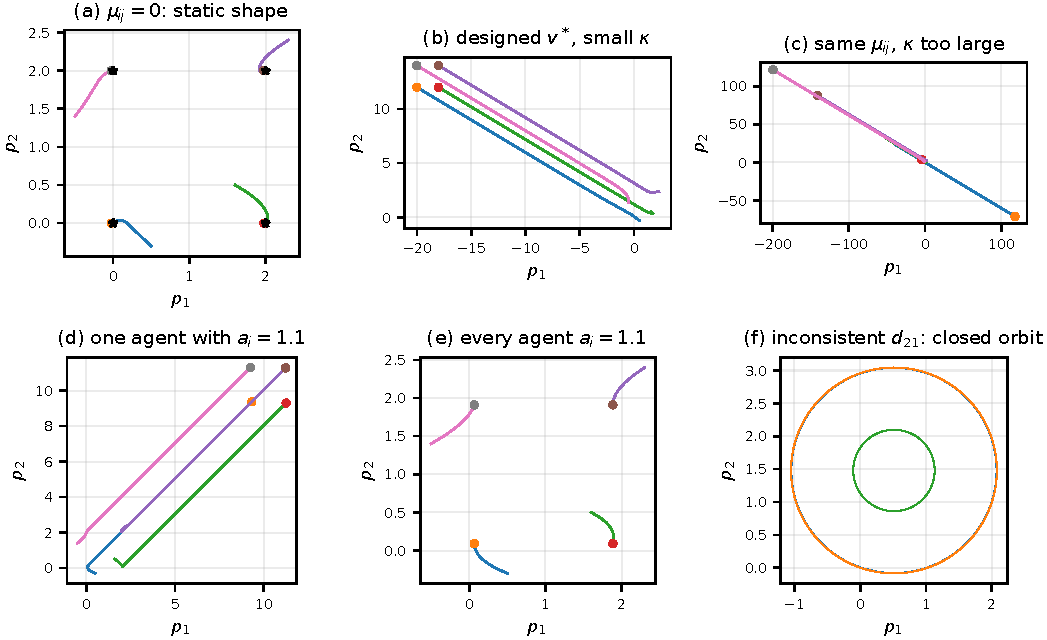
\includegraphics[width=\textwidth]{figures/fig-methods.pdf}
  \caption{两类文献机理的复现（$p_1,p_2$ 为平面坐标，圆点为末态）。
  (a) 位移一致性 $\mu_{ij}=0$：收敛到静态参考形状。
  (b) 设计机动（树图，$\kappa=1$）：四条轨迹成为平行直线，形状不变，实测公共速度
  $-\kappa v^*$（$v^*=(0.5,-0.3)$）。
  (c) 同一 $\mu_{ij}$、$\kappa=5$：形状失稳、边长从 $1.36$ 发散到 $143$，即
  \eqref{eq:kappa_bound} 所禁止的区域。
  (d) 位移一致性 $+$ 单个 agent 的尺度因子 $a_0=1.1$：形状扭曲但刚性，四车共享同一速度
  $\abs{v}=0.066$（离散度 $10^{-17}$），整体匀速平移。
  (e) 四个 agent 全部取 $a_i=1.1$：残余速度为零，形状静止且被统一缩放（$1.414\to1.286$）。
  (f) 距离梯度 $+$ 一条边的标准距离不一致（$6\%$）：边长收敛到恒定的 $1.0302$，三车各自沿
  半径 $0.583$ 的圆轨道以恒定速率 $0.0557$ 运动，即~\cite{tro2015} 的寄生闭合轨道。}
  \label{fig:methods}
\end{figure}

\subsection{把旋转设计出来：复平面相位加权一致性}
\label{sec:meth_designed}

上一小节说明位移一致性只允许平移。要\emph{设计}旋转，最干净的做法是换到复平面：取
$r_i,v_i,u_i\in\mathbb C$（虚数单位 $\mathrm j$ 即 $90^\circ$ 旋转算子 $J$），动力学仍是双积分器
$\dot r_i=v_i,\ \dot v_i=u_i$，并把转速 $\omega>0$ 作为\emph{给定常数}（可证不失一般性取 $\omega=1$）。
~\cite{lin2010} 的协议为
\begin{equation}
  u_i=\underbrace{\mathrm j\omega v_i}_{u_{i1}}
   -\sum_{k\in\calN_i}a_{ik}\rho_i^{-2}\Bigl[v_i-\frac{\rho_i}{\rho_k}
     \mathrm e^{\mathrm j(\theta_i-\theta_k)}v_k\Bigr]
   -\sum_{k\in\calN_i}a_{ik}\bigl(c_i-c_k\bigr),
  \qquad c_i=r_i+\omega^{-1}\mathrm j v_i ,
  \label{eq:linproto}
\end{equation}
期望构型写成极坐标 $h=[\rho_1\mathrm e^{\mathrm j\theta_1},\dots,\rho_n\mathrm e^{\mathrm j\theta_n}]^{\mathsf T}$，
其中 $c_i$ 是“圆心”，$\rho_i$ 是半径。三件事值得记下。

\paragraph{(i) 旋转来自前馈，而不是来自共识。}
$u_{i1}=\mathrm j\omega v_i$ 是\emph{纯向心加速度}：它让每辆车自己进入半径 $\norm{v_i}/\omega$、
圆心 $c_i$ 的圆周运动（$\dot v_i-\mathrm j\omega v_i\to0$）。共识项 $u_{i2}$ 只负责对齐
“圆心”与“相位加权速度” $v_i/(\rho_i\mathrm e^{\mathrm j\theta_i})$，形状与转速都不是共识
“涌现”的。这正是 \eqref{eq:disp} 所缺的那一半：平移机动用非对称 Laplacian 的常值特解
\eqref{eq:pparticular}，旋转机动用一个与速度垂直的前馈项，二者是同一种“把运动写进闭环”的思路。

\paragraph{(ii) 复增益等价于普通 Laplacian。}
取 $H=\mathrm{diag}\{\mathrm e^{\mathrm j\theta_i}\}$、$F=\mathrm{diag}\{\rho_i\}$，则耦合矩阵
$\tilde L_{ik}=\rho_i^{-1}\rho_k^{-1}\mathrm e^{\mathrm j(\theta_i-\theta_k)}l_{ik}$ 可写成
$\tilde L=F^{-1}HLH^{*}F^{-1}$，与 Laplacian $L$ 相合，故连通图上仍是“一个零特征值、其余正实部”。
闭环谱因此只有两个“保守”模态（特征值 $0$ 与 $\mathrm j\omega$，对应圆心一致与刚体旋转相位），
其余 $2n-2$ 个实部为负——需要一条排除广义特征向量与共线退化的假设（原文 Assumption~1）。
但这类协议只锁\emph{形状}：\cite{lin2010} 的 Remark~2 明确指出，最终构型的\emph{尺寸}由初值决定
（“quasi-rotating formation”）。

\paragraph{(iii) 半径靠一个估计器钉住。}
要得到尺寸也正确的旋转编队，需指定一个 agent $s_{i_0}$ 兼任幅值伺服：
\begin{equation}
  \dot p=\mathrm j p-\Lambda\sgn(\norm p-1)p
        -d\Bigl(p-\frac{v_{i_0}}{\rho_{i_0}\mathrm e^{\mathrm j\theta_{i_0}}}\Bigr),
  \qquad
  \Lambda=\frac{\kappa_1\norm p^2+\kappa_2}{\norm p^2},\quad \norm{p(0)}=1,
  \label{eq:linleader}
\end{equation}
并在 $u_{i_0}$ 中追加注入项 $\rho_{i_0}\mathrm e^{\mathrm j\theta_{i_0}}p-v_{i_0}$，其余 agent 仍用
\eqref{eq:linproto} 的 $u_{i2}$ 与 $\mathrm j\omega v_i$ 之和。用 $V_p=p^{*}p$ 可证：只要
$\kappa_1>d(\sqrt{V_0/\lambda_p}+1)$、$\kappa_2>2d+d\sqrt{V_0/\lambda_p}$，就有
$\norm{p(t)}\equiv1$，于是理想速度 $\rho_i\mathrm e^{\mathrm j\theta_i}p$ 的模恒为 $\rho_i$——
半径被钉死，尺寸不再依赖初值。稳定性则归结为一个 Lyapunov 不等式（存在正定 Hermite $\bar P$ 使
$\bar P\bar\Gamma+\bar\Gamma^{*}\bar P-d(\cdot)<0$，$\bar\Gamma$ 为去掉中性模态后的闭环矩阵）。

\paragraph{与本报告的关系。}
两条路线在“旋转”这一点上互为镜像，区别可以压缩成三句话。其一，\emph{转速从哪来}：
~\cite{lin2010} 的 $\omega$ 是设计参数（想快就调大，控制器里显式出现 $\mathrm j\omega v_i$），
而本报告的 $\abs{\omega}=\sqrt{k_2}$ 被“中心内力矩恒为零”与观测器积分钉死（命题~\ref{prop:omega}），
既不能设计也不能调参。其二，\emph{切向注入乘在谁身上}：\eqref{eq:linproto} 的 $\mathrm j\omega v_i$ 乘
\emph{自己的速度}，是前馈，效果是让每辆车在旋转坐标系里做静止调节；本报告稳态观测器给出
$\tv_i=\frac{k_2}{\omega}J\txi_i$，乘的是\emph{相对位置}，是反馈，效果是刚性形状整体转动。
其三，\emph{谁决定形状}：\eqref{eq:linproto} 的形状 $h$ 与半径都由设计者指定，而本报告的成对距离、
转速、旋转方向全部由闭环决定，只能证明局部轨道稳定（\S\ref{sec:stab}）。因此“把 $\omega$ 设计进去”
的办法无法解释围捕控制器为什么\emph{一定}转，也无法用来消掉这个旋转。

\subsection{鲁棒性：残余运动什么时候出现}
\label{sec:meth_robust}

同一框架下更微妙的问题是：\emph{感知不完美}时闭环是否还会停住。~\cite{tac2021} 采用的感知模型是
\begin{equation}
  (p_j-p_i)\big|_{\text{meas}}=a_iR_i\,(p_j-p_i),\qquad a_i>0,\ R_i\in SO(m),
  \label{eq:badsense}
\end{equation}
即每个智能体各有\emph{尺度因子} $a_i$ 与\emph{局部坐标系旋转} $R_i$（罗盘/航向偏置）。记
$D_x=\bar D_aD_R$，闭环变成 $\dot p=-D_x\bar Lp+\bar Lp^*$，与设计机动 \eqref{eq:modlap}
形式相似但本质不同：扰动直接乘在 Laplacian 上。

结论可以压缩成一句判据：\textbf{残余运动来自“分歧”，而不是“误差”}。若所有智能体的失配完全
相同（$a_i=a^*$、$R_i=R^*$），则残余速度为零，位置收敛到静态的、只是被统一缩放/旋转过的形状
\begin{equation}
  \tilde p^*=\frac{1}{a^*}\bigl(I_n\otimes R^{*\mathsf T}\bigr)p^*+\mathbf 1_n\otimes b ;
  \label{eq:trivial}
\end{equation}
只要有一个智能体的 $(a_i,R_i)$ 与他人不同，闭环就收敛到“扭曲的形状 + 常值残余速度”：
\begin{equation}
  \tilde z^*=\bigl(\bar B^{\mathsf T}D_x\bar B D_\omega\bigr)^{-1}\bar B^{\mathsf T}\bar BD_\omega z^*,
  \qquad
  D_x\bar L\tilde p^*-\bar Lp^*=-(\mathbf 1_n\otimes\tilde v^*).
  \label{eq:residual}
\end{equation}
~\cite{tac2021} 的定理 2 证明：图\emph{无环}（树）且至少有一个智能体的尺度或坐标系与他人不同、
$D_x\approx I$ 时，\eqref{eq:residual} 成立，编队以常速 $\tilde v^*$ 平移。带环图的相应结论
\emph{没有}被证明：$\bar B^{\mathsf T}\bar B$ 奇异使 \eqref{eq:residual} 的第一式不可直接求解，
只能先分解独立坐标；“$\tilde z^*\notin\ker\check M$（即 $\tilde v^*\neq0$）”被作者明确列为开
问题。这就是“树 vs 带环”的实质差别：树有闭式判据，带环只有部分结果。

图~\ref{fig:methods}(d)(e) 复现了这条判据。四车正方形环，仅让 $a_0=1.1$、其余为 $1$：形状收敛
到\emph{刚性但扭曲}的正方形（到质心距离 $1.414\to\{1.332,1.414,1.365,1.414\}$），四车共享同一个
速度 $\abs{v}=0.066$（车与车之间的离散度 $1.6\times10^{-17}$）。把四个 $a_i$ 全部取 $1.1$：残余
速度为零，形状静止，半径 $1.414\to1.286=1.414/1.1$，正好是 \eqref{eq:trivial}。

一个容易被误读的点值得说清：在这个\emph{位移一致性}框架里，残余运动是“扭曲形状的匀速平移”
（$\tilde v^*$ 是公共速度），并不自旋——我们的数值实验中每辆车的方位角变化为零。\emph{旋转型}
的残余运动出现在下一小节的\emph{距离}型闭环中（闭合圆轨道），以及罗盘失配类工作（如
~\cite{tac2021} 引用的 “mismatched compasses”）中；平移与转动同时出现的机动方案见
~\cite{tro2016}。

\subsection{距离梯度控制中的寄生旋转}
\label{sec:meth_parasitic}

最经典的“不该转却转了”是~\cite{tro2015}。距离梯度控制为
\begin{equation}
  u_i=-\sum_{k_{ij}\in\mathcal E_i}z_{ij}\,e_{k_{ij}},
  \qquad
  e_{k_{ij}}=\norm{z_{ij}}^2-d_{k_{ij}}^2 ,
  \label{eq:grad}
\end{equation}
即势函数 $\frac14\sum_k e_k^2$ 的梯度。当同一条边两端的“标准距离/实测距离”不一致
（$\bar d_{k_{ij}}\neq\bar d_{k_{ji}}$，等价地 $e_{k_{ij}}\neq e_{k_{ji}}$）时，
\eqref{eq:grad} 不再是任何单一势函数的梯度，于是出现两种不良行为：
\begin{enumerate}[leftmargin=2.2em]
  \item \emph{未知的扭曲终态形状}：$e_k$ 收敛到小的非零常值，形状被永久扭曲；
  \item \emph{稳态集体运动}：$\R^2$ 中整个编队沿一条闭合轨道运动，轨道由\emph{单一正弦信号}
        决定；$\R^3$ 中则变成螺旋（正弦 + 常值漂移）。
\end{enumerate}
这里的关键洞察是：\textbf{指数收敛只对“误差信号”成立}，它不允许我们推断位置或速度也收敛
——$e_k\to$ 常数并不排斥 $\dot p_i$ 停在非零值。这是梯度型编队控制被低估的鲁棒性陷阱。

图~\ref{fig:methods}(f) 是三车等边三角形的复现：把 $\bar d_{21}$ 从 $1$ 改成 $1.06$（$6\%$），
边长收敛到恒定的 $1.0302$（扭曲但刚性），三车各自在半径 $0.5829$ 的圆上以恒定速率 $0.0557$
运动（末段速率标准差 $1.6\times10^{-9}$），质心同时缓慢漂移——正是“刚性但扭曲 + 闭合轨道”。

消除办法是\emph{分布式内模估计器}~\cite{tro2015}。对每条边指定一个 estimating agent，把不一致
$\mu_k$ 建模为“常值 $+$ 有限个已知频率正弦”的外系统输出 $\mu_k(t)=\alpha_k+\sum_i\beta_i\sin(\omega_it+\phi_i)$，
用 $(\xi_k,\hat\mu_k)$ 估计它，并在控制中补偿：
\begin{equation}
  u_i=-\sum_{k_{ij}\in\mathcal E_i}z_{k_{ij}}e_{k_{ij}}
      +\sum_{k_{ij}\in\kappa_i}z_{k_{ij}}\hat\mu_k,
  \qquad
  \dot\xi_k=\Lambda\xi_k+\kappa B_k\bigl(e_{k_{ij}}+\mu_k-\hat\mu_k\bigr),
  \ \hat\mu_k=B_k^{\mathsf T}\xi_k .
  \label{eq:internalmodel}
\end{equation}
其定理 5.1 说：若
\begin{equation}
  Z=-R(z^*)R(z^*)^{\mathsf T}+R(z^*)S_1(z^*)^{\mathsf T}
  \label{eq:Zmat}
\end{equation}
在期望构型（$e=0$）处 Hurwitz，则存在 $\kappa^*,b^*$，只要增益足够大、$B_k$ 的振荡分量足够小，
闭环就有一个局部指数吸引的不变流形 $\mathcal Q=\{(w,x,\xi)\,|\,e=0,\ \xi=w\}$：形状指数收敛到
期望形状、$\hat\mu\to\mu$、并且 $\dot x\to0$（\emph{整个编队最终停住}）。该文还给出如何系统
地挑选 estimating agents（三角编队、以及由 Henneberg 插入生成的一类最小刚性图上有组合判据），
并用三台 e-puck 实验说明：不加估计器时机器人“永不停止”（速度始终不衰减），加了之后停住。

\subsection{二阶（双积分器）版本}
\label{sec:meth_second}

同样的现象在双积分器上重现~\cite{sun2017robust}。设 $\ddot p_i=-\gamma\dot p_i
-\sum_j e_{k_{ij}}(p_i-p_j)+\sum_{j\in\calN_i^-}\mu_{k_{ij}}(p_i-p_j)$，则小常值失配下：
距离误差指数收敛到非零常值；形状指数收敛到（扭曲的）刚性形状；而位置轨迹（stabilization 版）
或其\emph{速度}轨迹（flocking 版）收敛到 $\R^2$ 的圆轨道 / $\R^3$ 的螺旋轨道
（该文定理 3、4）。

值得与本报告第~\ref{sec:double} 节对照：那里的旋转\emph{不需要}任何失配——观测器
$\dot w_i=-k_3e_i$ 自己就制造了切向驱动力，转速由力矩平衡钉死为 $\sqrt{k_3/k_2}$；而这里的旋转
完全由失配提供动力，无失配时编队会停住。两者形式上都是“二阶系统 + 一个积分型的内部状态”，
但一个是\emph{结构性的精确解}，一个是\emph{扰动诱发的极限轨道}。

\subsection{三类机制的对比}
\label{sec:meth_table}

表~\ref{tab:methods} 把三类机制并排。可以看出它们在“旋转由谁供能”“速率由谁决定”“怎么消除”
三件事上完全不同。

\begin{table}[htbp]
\centering
\small
\caption{三类编队旋转机制的对照。}
\label{tab:methods}
\setlength{\tabcolsep}{4pt}
\renewcommand{\arraystretch}{1.15}
\begin{tabular}{>{\raggedright\arraybackslash}p{0.15\textwidth}
                >{\raggedright\arraybackslash}p{0.24\textwidth}
                >{\raggedright\arraybackslash}p{0.26\textwidth}
                >{\raggedright\arraybackslash}p{0.27\textwidth}}
\toprule
 & \textbf{(A) 设计机动} & \textbf{(B) 测量失配（寄生）} & \textbf{(C) 约束缺失（本报告）}\\
\midrule
控制框架 & 位移一致性 $+$ 修改 Laplacian & 距离/位移梯度 & 围捕控制器 \eqref{eq:ctrl7}\\
触发条件 & 人为取 $\mu_{ij}\neq\mu_{ji}$ & 端点标准或感知不一致（$a_i$、$R_i$、
            $\bar d_{k_{ij}}$ 有分歧） & 无需任何分歧：只约束平均\\
形状 & 严格保持 $\mathcal S$ & 扭曲但刚性（误差停在非零常值） & 刚性，成对距离收敛到常数\\
运动 & 匀速平移（公共 $v^*$）；旋转需另设机制，即复平面相位加权
           $+$ 前馈 $\mathrm j\omega v_i$~\cite{lin2010} & 2D 闭合圆轨道 / 3D 螺旋 / 扭曲形状的匀速平移 &
           绕目标的刚体旋转\\
速率由谁定 & 设计参数 $\kappa b$（旋转情形为 $\omega$~\cite{lin2010}） & 由失配量与闭环算子决定，一般无闭式 &
           力矩平衡强制 $\abs{\omega}=\sqrt{k_2}$\\
消除/避免 & 无需消除（$\kappa$ 需足够小，树图有界） & 内模估计器补偿 $\mu_k$，或一致化标定 &
           观测器中加入 $\phi_i$（\S\ref{sec:second}）\\
\bottomrule
\end{tabular}
\end{table}

\subsection{与围捕控制器的结构对应}
\label{sec:meth_relation}

把三类机制放在一起看，本报告的围捕控制器其实与 (A)、(B) 各有一半的“血缘”，但都不重合。

\paragraph{(i) 观测器 $=$ 相位滞后 $90^\circ$ 的切向注入。}
第一种控制器的观测器在旋转稳态上给出 $\tv_i=\frac{k_2}{\omega}J\txi_i$，即一个\emph{与相对
位置垂直}的速度分量，比例系数 $k_2/\omega$。这与 \eqref{eq:muJ} 中“把 $\mu$ 的反对称部分
$bJ$ 取出来”得到切向驱动的做法在形式上完全同型：围捕控制器相当于用\emph{积分器自动实现了
非对称权重}，不需要显式设计 $\mu_{ij}$。

\paragraph{(ii) 但速率的来源完全不同。}
设计中 $\mu_{ij}$ 的速率是自由参数（$\kappa b$），想快就调大；围捕控制器的速率却被闭环
\emph{强制}为 $\sqrt{k_2}$（命题~\ref{prop:omega}），既不能设计也不能调参改变——因为它是
“中心内力矩恒为零”这一几何事实与观测器积分的耦合结果。这正是本文旋转区别于文献机动方案的
本质：\emph{不是把旋转设计出来，而是发现旋转是唯一的自洽解}。

\paragraph{(iii) 消除手段的共同结构。}
~\cite{tro2015} 消除寄生轨道的方法是“用内模估计器把不一致显式补偿掉”，本报告消除旋转的方法
是“在观测器里加 $\phi_i$，让 $\dot V$ 成为负平方和”（\S\ref{sec:second}）。两者手法不同，
逻辑相同：把那个“没有被约束/被扰动的方向”显式地阻尼或补偿掉。反过来说，任何“只约束平均”
的设计都注定要面对一个类似的中性方向。

\paragraph{(iv) 互相不可替代。}
失配型旋转的前提是“分歧”：所有智能体一致地错（$a_i\equiv a^*$、$R_i\equiv R^*$）时残余运动
为零（\eqref{eq:trivial}）。围捕控制器的旋转不需要任何分歧——所有车辆对目标速度、对邻居距离的
认知完全一致，旋转来自\emph{约束的缺失}而不是\emph{感知的偏差}。因此 (A) 的“一致化标定/估计器”
处方对本文的旋转无效（标定得再准也会转），而本文的“观测器加 $\phi_i$”处方对失配型问题也没有
意义（那里本该静止却动了）。这也解释了为什么两类文献长期各自为政。



\section{长期行为：旋转／卡死／呼吸的三分法}
\label{sec:trichotomy}

命题~\ref{prop:omega} 只确定转速，第~\ref{sec:stab} 节只给出局部分支的稳定性。两者都不回答“长期
行为有哪几类”。数值证据指向三类吸引子，我们把它记为猜想。下列事实是严格的：平均误差指数收敛
（定理~\ref{thm:avg}）；$\alpha(s)\to+\infty$（$s\to d^+$）构成对数壁垒，故任意有限时间不会碰撞；
命题~\ref{prop:omega} 是旋转类的必要条件；共线子空间的卡死可以证明（命题~\ref{prop:jam}）。

\begin{conjecture}[三分法]
\label{conj:tri}
考察单积分器闭环（\eqref{eq:veh} 与 \eqref{eq:ctrl7}，$k_1,k_2>0$，斥力幅值取 \eqref{eq:alpha}）。
若初值无碰撞，即满足
\begin{equation*}
  \min_{i\ne j}\norm{x_i(0)-x_j(0)}>d ,
\end{equation*}
则其形状轨迹 $\ts(t)$ 的 $\omega$-极限集有界，且恰属于下列三个互不相交的类之一：
\begin{enumerate}[leftmargin=2.2em]
  \item \emph{旋转平衡轨道}：绕目标的非退化刚体旋转，$|\omega|=\sqrt{k_2}$，所有成对距离收敛到
        有限常数 $d_{ij}^*>d$（一般情形）；
  \item \emph{卡死边界}：至少一对距离趋于碰撞距离 $d$，位置收敛而观测器状态线性发散；
  \item \emph{呼吸极限环}：形状变量的非平凡周期轨道，$\ts(t+T)=\ts(t)$，所有成对距离始终严格
        大于 $d$ 但周期振荡；角速度与个体半径沿环变化。
\end{enumerate}
三种情形下平均位置误差都指数收敛到零，故编队中心都锁定到目标上。
\end{conjecture}

\begin{proposition}[共线子空间中的卡死]
\label{prop:jam}
把闭环限制在不变共线子空间（所有位置、目标、初始观测器误差共线）。设 $k_1,k_2>0$、初始间距
$>d$，则形状轨迹收敛 $\ts(t)\to\xi^*$，$\xi^*\ne0$，且至少一对间距趋于 $d$；同时
$\norm{\tvs(t)}\to\infty$ 线性发散。
\end{proposition}
证明要点：一维中每条边只有径向方向且 $\Phi''(s)=\alpha'(s)=-1/(s-d)^2<0$，故
$\nabla^2P\preceq0$、$B\succeq k_1I\succ0$，于是 $\dot E\le-k_1\norm{\dot\ts}^2\le0$，积分得
$\dot\ts\in L^2$，结合 $\ddot\ts$ 有界推出 $\dot\ts\to0$、$\ts\to\xi^*$。内部不存在平衡点：观测器静止
要求 $\txi_i=0$（全部塌到目标），被壁垒禁止，故 $\xi^*\ne0$、$\dot\tvs=-k_2\txi\to-k_2\xi^*\ne0$，
$\tvs$ 线性发散。位置有界而观测器发散，要求斥力幅值无界，故必有间距趋于 $d$。

\begin{remark}[逼近壁垒的速率]
把上述平衡投影到趋于 $d$ 的那条边的轴向，记 $c^*=k_2\abs{\langle\xi^*,e\rangle}>0$，则首阶平衡为
$\alpha(s(t))\sim c^*t$，配合 $\alpha(s)=1/(s-d)-1/(\mu-d)$ 得
\begin{equation}
  s(t)-d\ \sim\ \frac{1}{c^*t}\ \longrightarrow\ 0 ,
  \label{eq:jamrate}
\end{equation}
即间距以 $1/t$ 速率贴向壁垒，同时观测器状态线性发散。
\end{remark}

\paragraph{完整证明为何困难。}
命题~\ref{prop:jam} 之所以成立，是因为共线情形下阻尼矩阵正定。二维中 $B=k_1I-\nabla^2P$ 在旋转
平衡点之外变号：径向带 $\alpha'(s)<0$（阻尼），切向刚度 $\alpha(s)/s>0$ 贡献反阻尼——恰是维持旋转
的那一项。因此形状能量不是全局 Lyapunov 函数，目前也没有能把旋转吸引子与卡死吸引子分开的单调量；
而卡死分支位于向量场奇异的边界 $s=d$ 上，标准收敛定理不适用。

\paragraph{数值注意。}
壁垒使问题刚性化：贴近 $s=d$ 时局部时间尺度 $s-d\to0$ 而刚度 $\abs{\alpha'(s)}=1/(s-d)^2\to\infty$。
定步长显式格式会在壁垒附近爆掉，从而\emph{错误地}表现为发散或大幅振荡；必须用隐式/刚性求解器
（BDF、LSODA，容差 $10^{-8}$–$10^{-12}$）。同理，测量角速度时要注意分母 $\norm{\txi_i}^2$：
车辆靠近目标时 $\omega_i$ 会虚假增大，有意义的刚性旋转诊断应同时报告平均角速度、离散度
$\max_i\omega_i-\min_i\omega_i$ 以及全部成对距离。

\section{数值仿真}
\label{sec:sim}

本节的全部插图由同目录下的 \texttt{scripts/} 自动生成
（\texttt{fencing\_lib.py} 为闭环与被测度量，\texttt{make\_figures.py} 生成图片，
\texttt{summarize.py} 打印正文引用的数字）。默认参数取原文算例
\[
  N=6,\quad d=5,\quad \mu=9,\quad k_1=k_2=0.5,\quad
  v_0=(1,0)^{\mathsf T},
\]
初值为绕目标半径 $8$ 的正六边形、$v_i(0)=0$；积分在目标坐标系 \eqref{eq:rel} 中进行，
用 LSODA（刚性分支见 \S\ref{sec:sim_jam} 用 BDF），相对容差 $10^{-8}$–$10^{-9}$。
下文凡称“锁定”均指：末段 $25\%$ 时间窗内每辆车的角速度
$\omega_i=(\txi_i\times\dot\txi_i)/\norm{\txi_i}^2$ 的均值与末期值相差小于 $10^{-3}$。

\subsection{一维基准：静态编队}
图~\ref{fig:1d} 给出无观测器的朴素情形 $u_i=\phi_i+k_1(x_0-x_i)$（$N=5$，$d=0.5$，$\mu=2$，
$k_1=1$）。车辆在目标坐标系中收敛到静态编队，目标始终位于最小与最大位置之间（围捕成立），
最小间距稳定在 $d$ 之上。这是后续旋转判据的“平凡对照”：一旦观测器存在，静态编队就不再可能
（命题~\ref{prop:omega} 的第 0 步）。

\begin{figure}[htbp]
  \centering
  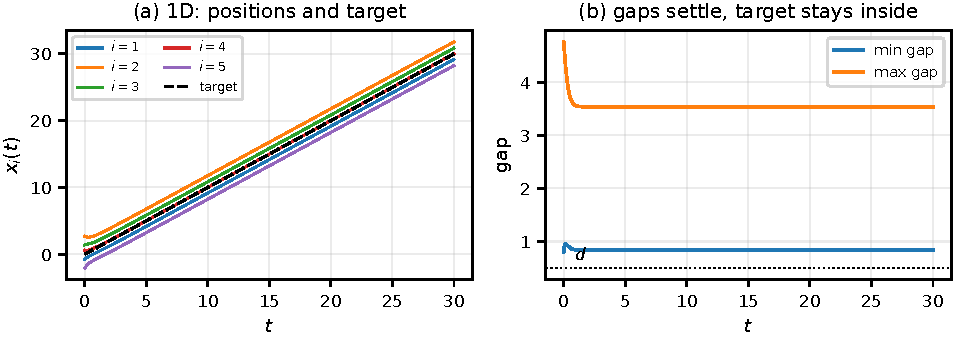
\includegraphics[width=0.95\textwidth]{figures/fig1d.pdf}
  \caption{一维基准（无观测器）。左：车辆位置与运动目标；右：最小/最大成对间距，收敛到常数并
  始终大于 $d$。目标被围在凸包内部，速度误差趋于零。}
  \label{fig:1d}
\end{figure}

\subsection{二维刚体旋转与角速度}
图~\ref{fig:rot} 是基准实验。末段 $25\%$ 时间窗内实测
$\bar\omega=-0.707107$，与 $\sqrt{k_2}=0.707107$ 吻合到 $10^{-7}$，个体离散度
$\max_i\omega_i-\min_i\omega_i=4.9\times10^{-8}$，成对间距收敛到
$\{5.471,5.881,9.707,10.932\}$（全部 $>d$）。
图~\ref{fig:rot}(b)(c) 正是第~\ref{sec:avg} 节的结构性事实：成对间距与\emph{平均}速度误差
都收敛，而\emph{个体}速度误差保持非零——末段其均值 $3.4319$ 等于 $\sqrt{k_2}\cdot\frac1N\sum_i\norm{\txi_i}$，
即纯切向。

\begin{figure}[htbp]
  \centering
  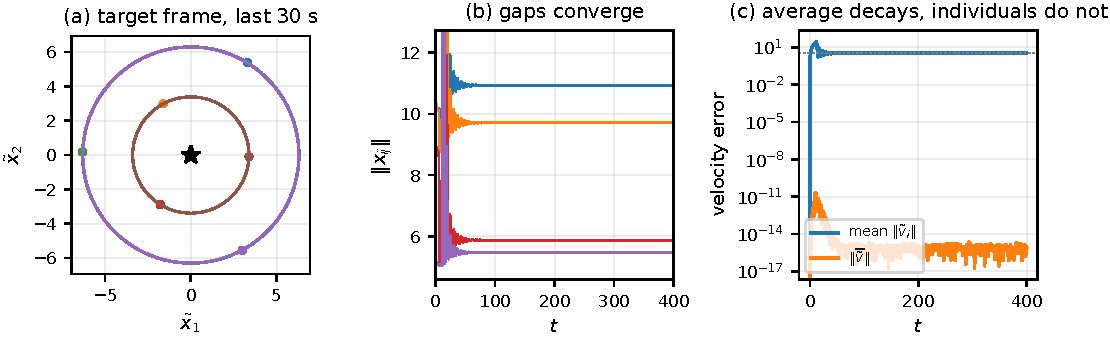
\includegraphics[width=\textwidth]{figures/fig2d-rotation.pdf}
  \caption{二维刚体旋转（$N=6$，$k_1=k_2=0.5$）。(a) 目标坐标系中末 $30$ s 的轨迹与末期位置；
  (b) 成对间距收敛到常数；(c) 平均速度误差指数衰减到 $10^{-17}$，而个体速度误差保持有界非零
  （虚线为 $\sqrt{k_2}\,\overline{\norm{\txi_i}}$）。}
  \label{fig:rot}
\end{figure}

图~\ref{fig:sweep} 把 $k_2$ 扫过 $0.05$–$2.0$（$40$ 倍）。$|\omega|$ 与 $\sqrt{k_2}$ 的相对误差
除了 $k_2=0.05$（$2.4\times10^{-5}$，慢收敛暂态尚未完全结束）以外都在 $10^{-9}$–$10^{-6}$，
远小于命题~\ref{prop:omega} 的检验门槛；这说明转速的选择与半径、形状、稳定性无关。

\begin{figure}[htbp]
  \centering
  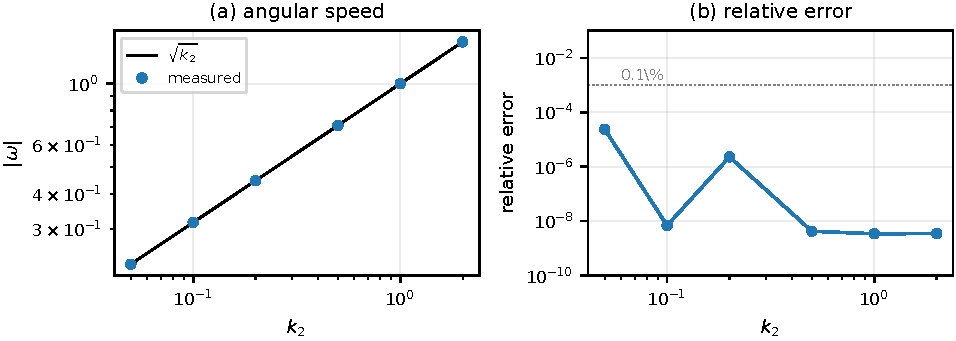
\includegraphics[width=0.95\textwidth]{figures/fig2d-omega-sweep.pdf}
  \caption{角速度选择定理的数值验证。(a) 实测 $|\omega|$ 与 $\sqrt{k_2}$（双对数）；
  (b) 相对误差，全部低于 $10^{-4}$，点线为 $0.1\%$ 参考。}
  \label{fig:sweep}
\end{figure}

\subsection{旋转形状：不是正六边形}
尽管初值是正六边形，稳态却是半径交替的交错双三角形：三个车在 $r=3.395$，三个在 $r=6.312$
（图~\ref{fig:branch}a）。而径向平衡的正六边形分支根为 $\alpha(r)=k_1r$ 的唯一解
$r^*=5.3423$（图~\ref{fig:branch}b 的虚线圆），\emph{并未}被选中。六辆车共享同一个
$\sqrt{k_2}$：零力矩恒等式在确定 $\omega$ 之前就把所有半径消掉了，这与
\S\ref{sec:omega} 末尾的论断一致。

\begin{figure}[htbp]
  \centering
  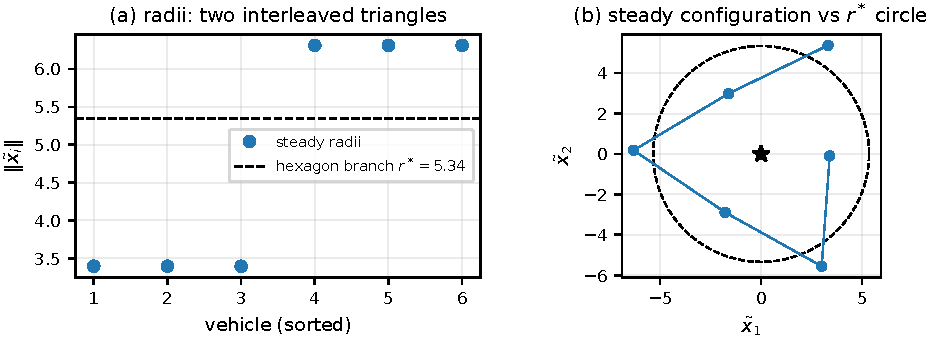
\includegraphics[width=0.95\textwidth]{figures/fig2d-shape-branch.pdf}
  \caption{旋转形状的分支选择。(a) 稳态半径按大小排序，呈 $3.395/6.312$ 交替；
  (b) 稳态构型与正六边形分支圆 $r^*=5.34$ 的对比：实际吸引子是交错双三角形。}
  \label{fig:branch}
\end{figure}

\subsection{退化子空间：只有真正不变的方向才不旋转}
命题~\ref{prop:omega} 是必要条件，因此“某些初值不旋转”是\textbf{在精确算术下}成立。
图~\ref{fig:deg} 把三种初值放在一起：共线初值（全部落在 $x$ 轴上）是有向环量
$L\equiv0$ 的\emph{精确}不变子空间，$y$ 分量在浮点运算下也恒为零，最终以 $1/t$ 速率卡死
（\S\ref{sec:sim_jam}）；而“四车置于坐标轴”（正方形）虽然 $L(0)=0$ 且关于两轴对称，却只是
\emph{精确算术下}不变——舍入噪声在 $t\approx20$ s 后被放大，$L$ 收敛到 $-44.8$，编队进入刚体
旋转（半径 $3.98$）；一般初值则给出 $L\approx-109$。这说明第~\ref{sec:dir} 节所说的“对称
子空间”在数值上并不稳健，只有与坐标轴严格对齐的共线子空间才是真不变的。

\begin{figure}[htbp]
  \centering
  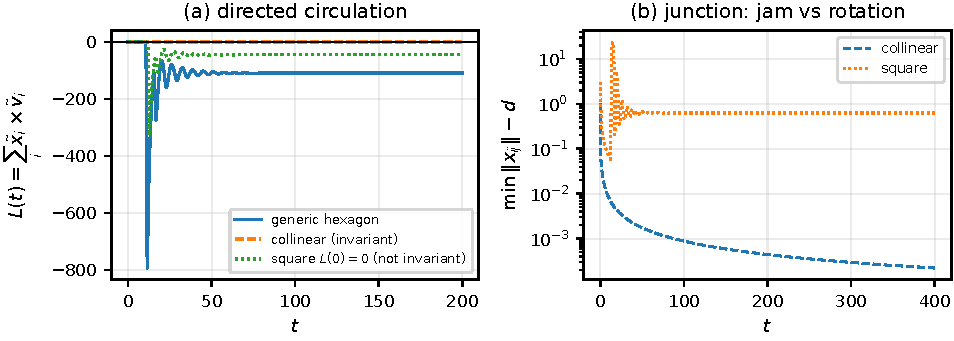
\includegraphics[width=0.95\textwidth]{figures/fig2d-degenerate.pdf}
  \caption{退化子空间的数值行为。(a) 有向环量 $L(t)$：共线初值恒为零，正方形初值被舍入噪声
  激活后锁定到刚体值，一般初值收敛到 $\omega\sum_i\norm{\txi_i}^2$；(b) 最小间距偏离 $d$ 的
  量：共线分支以 $1/t$ 贴向壁垒，正方形分支收敛到常数（即旋转而非卡死）。}
  \label{fig:deg}
\end{figure}

\subsection{局部稳定性的谱检验}
在数值求得的旋转平衡点上，把状态搬到共旋系并按 \eqref{eq:DF} 组装
$DF$（形状子空间维数 $2(N-1)=10$，故 $DF$ 为 $20\times20$；$\nabla^2P$ 由
$\Phi'=\alpha$、$\Phi''=-1/(s-d)^2$ 解析组装后在零均值子空间上投影）。结果与
\S\ref{sec:stab} 的预言逐项吻合（图~\ref{fig:spec}）：谱中恰有\emph{一个}零特征值，其模
$<3\times10^{-6}$，对应特征向量与 $(J\xi^*,-\omega_s\xi^*)$ 的对齐度在六位有效数字上等于
$1.000000$；其余全部严格在左半平面，谱横坐标为
\[
  k_2=0.1:\ -0.0156,\qquad
  k_2=0.2:\ -0.0312,\qquad
  k_2=0.5:\ -0.0780,\qquad
  k_2=1.0:\ -0.1557 .
\]
即衰减率随 $k_2$ 单调增大、且大致与 $\omega=\sqrt{k_2}$ 同阶：小增益下起旋暂态极慢，这与
\S\ref{sec:sim} 开头对收敛时间的观察一致。

\begin{figure}[htbp]
  \centering
  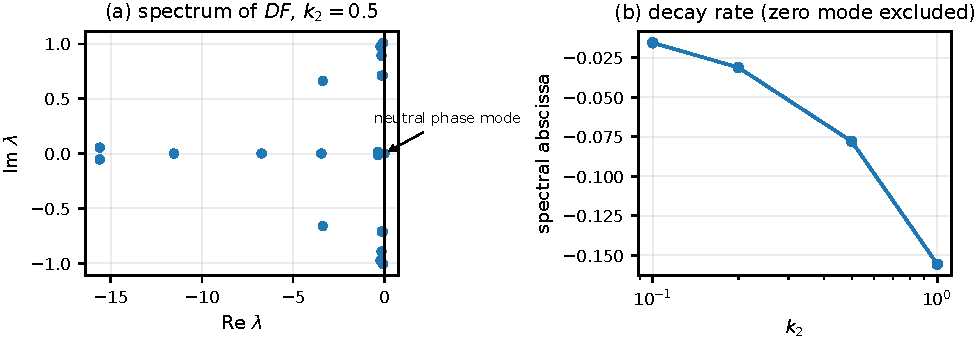
\includegraphics[width=0.95\textwidth]{figures/fig2d-spectrum.pdf}
  \caption{共旋线性化的谱（$k_2=0.5$，$20\times20$）。(a) 特征值实部/虚部：只有 $0$ 处一个
  中性相位模，其余严格在左半平面；(b) 去掉零模后的谱横坐标随 $k_2$ 的变化。}
  \label{fig:spec}
\end{figure}

\subsection{方向选择：符号由初始环量决定}
以切向小扰动 $v_i(0)=\varepsilon J x_i(0)$（故 $\sgn L(0)=\sgn\varepsilon$）扫描
$\varepsilon\in\{\pm10^{-2},\pm10^{-6},\pm10^{-12}\}$：每一次都锁定到
$|\omega|=0.707107$、且 $\sgn\omega=\sgn\varepsilon$（图~\ref{fig:dir}a），锁定时刻在
$86$–$91$ s 之间，与 $|\varepsilon|$ 跨越十个数量级无关。也就是说，环量的\emph{大小}
只决定放大所需时间（差异不到 $6\%$），\emph{符号}决定吸引子。

零环量的对称初值是临界情形。图~\ref{fig:dir}(b) 追踪 $|L(t)|$：它从舍入噪声量级
（$\sim10^{-14}$）指数增长，约 $t\approx100$–$300$ s 后饱和到刚体值
$|L|=\sqrt{k_2}\sum_i\norm{\txi_i}^2=108.96$，末段 $\bar\omega=-0.707107$、个体离散度
$3.6\times10^{-11}$。因此本算例中对称流形\emph{确实是}排斥的，只是排斥很弱、锁定很晚。

\begin{remark}[“对称初值不旋转”只在精确算术下成立]
严格说，$L(0)=0$ 与关于某轴的反射对称性只能保证\emph{精确}解留在该子空间内；数值上该子空间
是排斥的，指数增长率即 \eqref{eq:DF} 中最接近虚轴的非零模的实部。本算例的增长率约为
$\lambda\approx0.1$–$0.2$，从 $10^{-16}$ 放大到 $O(1)$ 需要 $200$–$400$ s，与图~\ref{fig:dir}(b)
的饱和时刻相符。
\end{remark}

\begin{remark}[与更早一次实验的差别]
早先的一次同类实验（$6000$ s 视界）报告称对称初值始终未锁定，只保留了一个符号确定的
非刚性环流。与图~\ref{fig:dir}(b) 的差别不在于物理，而在于扰动的初始幅度：对称流形上的
增长率为某个正实数 $\lambda$，锁定时间 $\sim\lambda^{-1}\ln(1/\delta)$，$\delta$ 是舍入噪声
或积分器容差引入的不对称量。换机器、换容差、换求解器都会改变 $\delta$，从而改变锁定时间；
这正是原文图 2--4 中“旋转方向不可复现”的根源。
\end{remark}

\begin{figure}[htbp]
  \centering
  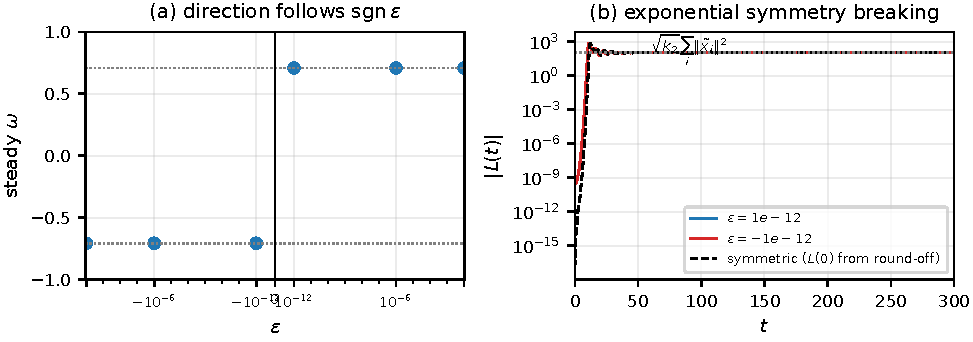
\includegraphics[width=\textwidth]{figures/fig2d-direction.pdf}
  \caption{方向选择。(a) 稳态 $\omega$ 与 $\varepsilon$ 的关系（symlog 横轴）：符号完全跟随
  $\sgn\varepsilon$，幅值恒为 $\sqrt{k_2}$；(b) $|L(t)|$ 从舍入噪声指数放大到刚体值
  $\sqrt{k_2}\sum_i\norm{\txi_i}^2$：$\varepsilon=\pm10^{-12}$ 与完全对称（虚线）三条曲线重合。}
  \label{fig:dir}
\end{figure}

\subsection{呼吸极限环与多吸引子}
用 Case C 初值（$N=5$，$k_1=k_2=0.5$，非对称）积分 $600$ s，末段成对间距持续周期振荡而
不收敛（图~\ref{fig:breath}a）：主导频率 $f=0.4032$ Hz，即周期 $T=2.4804$ s，有效频率比
\[
  \frac{\omega_{\text{eff}}}{\sqrt{k_2}}=\frac{2\pi f}{\sqrt{k_2}}=3.582,
\]
与“径向模被斥力刚度加硬”的图像一致：$\omega_{\text{eff}}^2=k_2+C_{\text{rep}}$，
$C_{\text{rep}}/k_2\approx 11.8$。最小间距在末段为 $5.245$（始终 $>d$），但各对间距的振荡幅度
差异极大（$0.2$ 到 $5.5$），说明这不是整体均匀的“呼吸”，而是形状层面的复杂周期运动；
对应地 $\bar\omega=-0.684$ 而个体离散度高达 $2.57$——\emph{不是}刚体旋转（图~\ref{fig:breath}c）。

\begin{figure}[htbp]
  \centering
  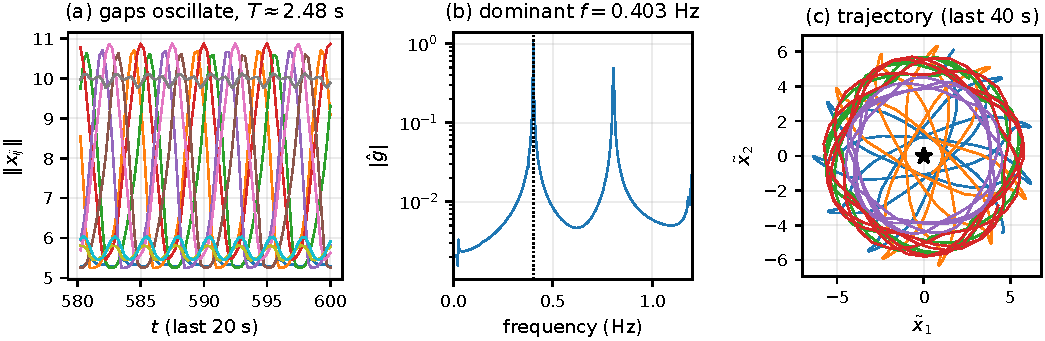
\includegraphics[width=\textwidth]{figures/fig2d-breathing.pdf}
  \caption{二维呼吸极限环（Case C，$N=5$，$k_1=k_2=0.5$）。(a) 末 $20$ s 的成对间距，周期
  $T\approx2.48$ s；(b) 间距序列的频谱，主峰 $f=0.403$ Hz；(c) 末 $40$ s 的轨迹：各车绕目标
  的非刚性周期运动。}
  \label{fig:breath}
\end{figure}

同一组增益下，正六边形初值走向刚体旋转、Case C 走向呼吸极限环，这就是双稳态
（图~\ref{fig:bist}a）。增大 $k_1$ 会消灭极限环：$k_1=0.3$ 与 $0.5$ 时仍呼吸，而 $k_1=0.7$ 时
间距收敛到常数 $5.6$，即转成 $\omega=\sqrt{k_2}$ 的刚体旋转（图~\ref{fig:bist}b）。这与原始
笔记中鞍结分岔的临界点 $k_1^{\text{crit}}\approx0.65$ 相符。

\begin{figure}[htbp]
  \centering
  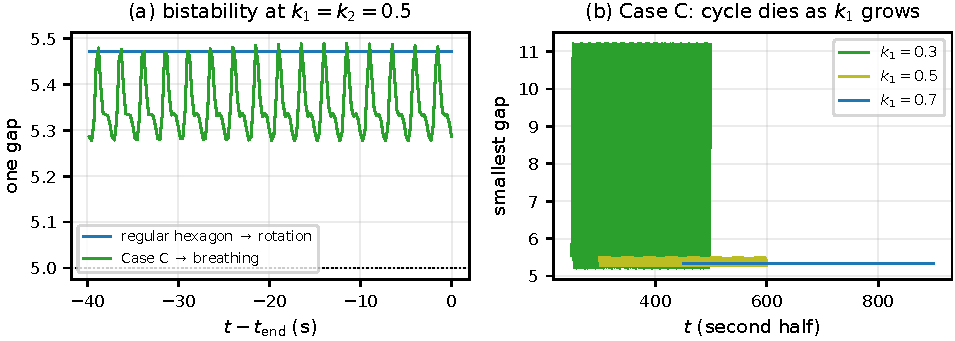
\includegraphics[width=0.95\textwidth]{figures/fig2d-bistability.pdf}
  \caption{双稳态与极限环的消失。(a) 同一组增益、两种初值：正六边形收敛到常数间距，Case C
  持续振荡；(b) Case C 初值在 $k_1=0.3,0.5$ 下呼吸，在 $k_1=0.7$ 下收敛到常数间距（刚体旋转）。}
  \label{fig:bist}
\end{figure}

\subsection{三维与非平面呼吸}
把同一闭环放到 $\R^3$（目标速度 $v_0=(1,0,0)$）：随机三维初值收敛到\emph{非平面}呼吸，
成对间距的谱峰在 $f=0.2197$ Hz（$T=4.551$ s），用末段位置协方差的奇异值比度量非平面性，
$\sigma_3/\sigma_1=0.863$（图~\ref{fig:3d}a,c）。而以平面正六边形初值时，$z$ 分量在整个
积分过程中恒为 $0$（$|z|_{\max}=0$），编队保持平面并以 $\omega=-0.707107$ 旋转，
个体离散度 $9.4\times10^{-8}$（图~\ref{fig:3d}b 的平线）。于是一维、二维、三维的图景统一：
刚性旋转要求形状落在低维不变子空间内，而高维自由度一旦被激发，就转而进入呼吸/锁频的周期
运动。

\begin{figure}[htbp]
  \centering
  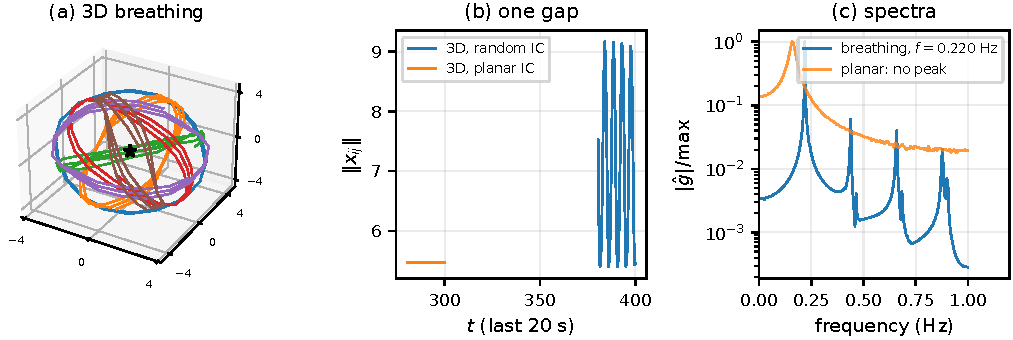
\includegraphics[width=\textwidth]{figures/fig3d-breathing.pdf}
  \caption{三维情形。(a) 随机三维初值末 $25$ s 的轨迹（三个坐标轴即 $\txi_i$ 的三个分量，明显非平面）；
  (b) 同一对车辆的间距：随机初值振荡，平面初值为常数；(c) 间距的频谱：前者在
  $0.22$ Hz 有主峰，后者无峰。}
  \label{fig:3d}
\end{figure}

\subsection{规模 $N$ 与斥力函数形式}
图~\ref{fig:ns} 用 \texttt{data/n\_scaling\_results.json}（$N=3,\dots,35$ 的旧扫描结果）（$k_1=k_2=0.5$，$\mu$ 随 $N$ 缩放）把每个
车辆相对编队中心的运动分解为径向（呼吸）与切向（旋转）两个频率。可以看到两个区制：
小 $N$ 时 $f_{\text{tan}}\approx f_{\text{rot}}=\sqrt{k_2}/(2\pi)$ 而 $f_{\text{rad}}/f_{\text{rot}}=1.4$–$1.9$
（呼吸区，切向仍是中性模）；$N\ge15$ 时两个模态\emph{锁频}，
$f_{\text{rad}}=f_{\text{tan}}\approx(1.5$–$1.8)f_{\text{rot}}$（锁定区），切向频率被斥力刚度
显著推离 $\sqrt{k_2}$。非平面性随 $N$ 增大迅速饱和到 $\sigma_3/\sigma_1\approx0.8$–$0.9$。

\begin{figure}[htbp]
  \centering
  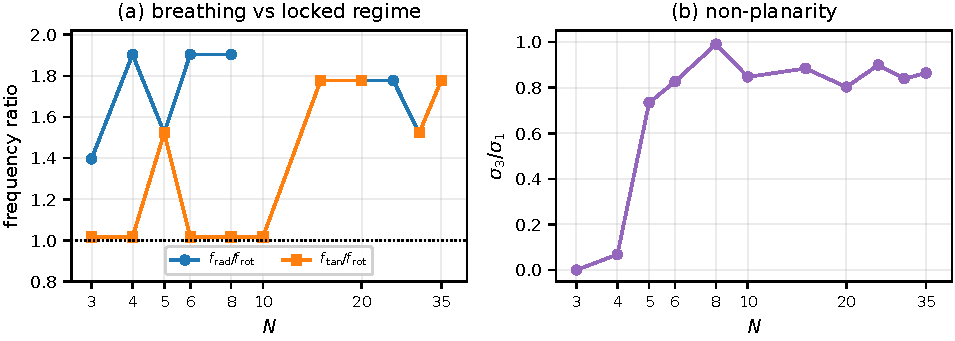
\includegraphics[width=0.95\textwidth]{figures/fig-nscaling.pdf}
  \caption{规模效应（$k_1=k_2=0.5$）。(a) 径向/切向频率与刚体旋转频率之比：$N\le8$ 时切向频率
  即 $\sqrt{k_2}/(2\pi)$，$N\ge15$ 时两模态锁频并整体上移；(b) 非平面性随 $N$ 的饱和。
  （$N=10$ 的径向与 $N=25$ 的切向为近直流 FFT 伪值，已略去。）}
  \label{fig:ns}
\end{figure}

图~\ref{fig:alpha} 比较六种连续化的斥力幅值（\texttt{data/alpha/}）（标准、幂、有理、对数、二次、指数；均满足
$\alpha(s)\to\infty$（$s\to d^+$）、$\alpha=0$（$s>\mu$））。对 $k_2\ge0.3$，六条周期曲线
几乎重合成 $T\approx0.52\cdot2\pi/\sqrt{k_2}$，只有 $k_2$ 很小时指数型偏离（其奇异项更强，
把呼吸推慢）；而呼吸\emph{强度}（频谱峰值比）随形式变化很大（$0.37$–$0.93$）。因此“周期由
$k_2$ 决定”是结构性质，而“呼吸多强”才是斥力函数设计可以调节的量。

\begin{figure}[htbp]
  \centering
  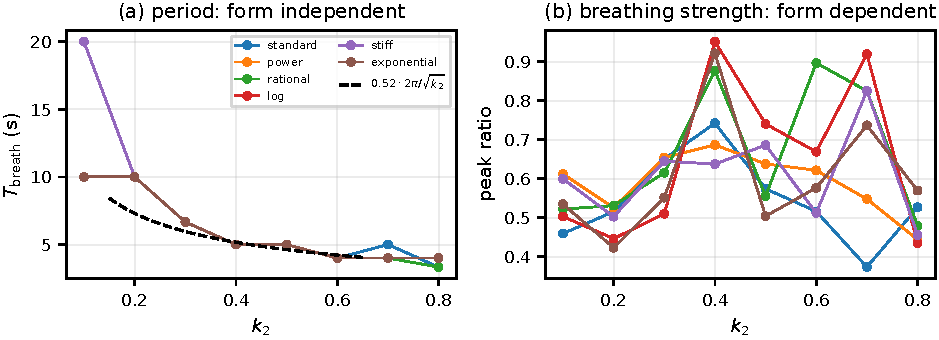
\includegraphics[width=0.95\textwidth]{figures/fig-alpha.pdf}
  \caption{六种连续 $\alpha$ 形式的比较。(a) 呼吸周期：$k_2\ge0.3$ 时六条曲线重合，并与
  $0.52\cdot2\pi/\sqrt{k_2}$（虚线）一致；(b) 呼吸强度：随形式差异显著。}
  \label{fig:alpha}
\end{figure}

\subsection{双积分器的数值检查}
对双积分器闭环 \eqref{eq:dctrl}（$k_1=0.5$，$k_3=0.2$，$N=6$），把初值放在
\S\ref{sec:double} 的径向平衡给出的正六边形平衡上（$v_i(0)=\omega Je_i$，$w_i(0)=\frac{k_3}{\omega}Je_i$），
扫描 $k_2=0.5,0.6,0.8,1.0,1.5$。实测 $|\omega|$ 与 $\sqrt{k_3/k_2}$ 相符到
$3\times10^{-4}$ 以内（其中四个点相符到 $10^{-6}$），验证了命题~\ref{prop:domega} 与
速率律。图~\ref{fig:double}(b) 同时暴露出一件与单积分器相同的事：正六边形虽是径向平衡，
却是\emph{不稳定}的，$k_2=0.8$ 时它在 $t\approx100$ s 后分裂成半径 $4.70$ 与 $6.29$ 的
双三角形，而 $\omega$ 保持 $\sqrt{k_3/k_2}$ 不变——又一次说明“速率被强制、形状不被强制”。
需要说明的是，这些运行以预测平衡为初值，检验的是\emph{自洽性与速率律}，而非吸引性
（从远处出发的强坍缩在该系统里极度刚硬，见 \S\ref{sec:sim_jam} 的注记）。

\begin{figure}[htbp]
  \centering
  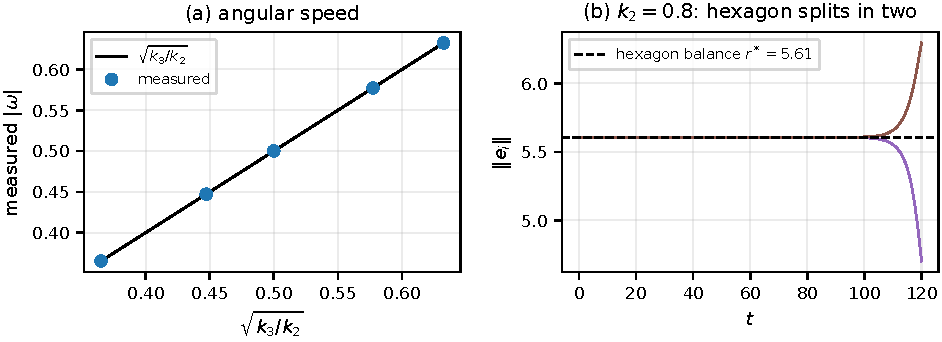
\includegraphics[width=0.95\textwidth]{figures/fig-double.pdf}
  \caption{双积分器（$k_1=0.5$，$k_3=0.2$）。(a) 实测 $|\omega|$ 与 $\sqrt{k_3/k_2}$；
  (b) $k_2=0.8$ 时各车半径：正六边形平衡（虚线）在 $t\approx100$ s 后分裂为两个三角形。
  }
  \label{fig:double}
\end{figure}

\subsection{卡死分支的 $1/t$ 律}
\label{sec:sim_jam}
共线初值（$N=6$，$x=\{-15,-9,-3,3,9,15\}$）用 BDF 积分到 $400$ s：最小间距单调贴向 $d$，
观测器范数以 $\norm{\tv}\propto t$ 线性发散（图~\ref{fig:jam}b：$t=50$ 时 $524$，$t=400$ 时
$4185$）。把间距代入 \eqref{eq:jamrate}，$(\min_{i\ne j}\norm{x_{ij}}-d)\,t$ 在整个区间上为
$0.0869\to0.0886$，即 $1/t$ 律在 $50$–$400$ s（近一个数量级）内成立，与
命题~\ref{prop:jam} 的注记一致；系数 $c^*$ 的首阶估计（$c^*\approx0.089$，而
$k_2\abs{\langle\xi^*,e\rangle}$ 给出同量级）也相符。这里必须用刚性求解器：显式格式在
$s\to d^+$ 处会因 $\abs{\alpha'(s)}=1/(s-d)^2\to\infty$ 而爆掉，把收敛误判为发散。

\begin{figure}[htbp]
  \centering
  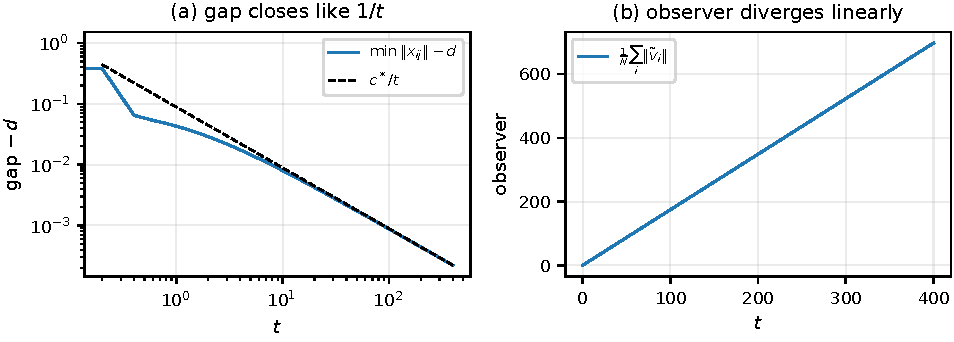
\includegraphics[width=0.95\textwidth]{figures/fig-jam.pdf}
  \caption{共线卡死分支。(a) 最小间距偏离 $d$ 的量（双对数）与 $c^*/t$ 参考线：$1/t$ 律在近一个
  数量级上成立；(b) 观测器状态线性发散。}
  \label{fig:jam}
\end{figure}


\section{结论与开放问题}
\label{sec:concl}

\begin{enumerate}[leftmargin=2.2em]
  \item \textbf{机理。}控制器只约束平均位置误差与平均速度，剩下 $2(N-1)$ 个环流自由度不受平均动力学
        约束。这些模态并非无阻尼（$k_1I$ 阻尼所有方向），而是径向平衡时斥力的切向刚度沿旋转方向
        恰好抵消 $k_1$，只留下一个中性模态（旋转相位），其余模态严格衰减。积分观测器把旋转的
        位置误差转成切向速度（或加速度），维持圆周运动。
  \item \textbf{频率选择。}中心斥力的零力矩恒等式强制 $\omega=\sqrt{k_2}$（单积分器）或
        $\omega=\sqrt{k_3/k_2}$（双积分器），与半径和形状无关。
  \item \textbf{有界性。}个体位置误差有界，且分离情形下可给出只依赖参数与初值的显式界；共线情形可给
        出全局显式界。
  \item \textbf{局部轨道稳定。}形状子系统为
        $\ddot\ts+B(\ts)\dot\ts+k_2\ts=0$，旋转协变使 $J\ts$ 在径向平衡处成为 $B$ 的零模；共旋线性化
        除一个零相位模外谱横坐标为负。全局证明受阻于 $B$ 在远离平衡点处变号。
  \item \textbf{方向选择。}旋转稳态上 $\sgn L=\sgn\omega$；任何非零初始环量（直到 $10^{-12}$）都唯一
        决定旋转方向，且锁定时刻几乎与幅值无关。零环量的对称初值只对应一个\emph{精确算术下}才不变
        的子空间：浮点舍入按指数律放大，约 $10^2$ s 后仍锁定到某个镜像刚体旋转，方向由噪声决定
        （因此不可复现）；只有与坐标轴严格对齐的共线子空间是真正不变、且必然卡死的一类。
  \item \textbf{消除旋转。}在观测器中加入 $\phi_i$ 使 $\dot V$ 成为负平方和，耗散每个个体的速度误差，
        得到刚性不旋转编队。
  \item \textbf{开问题。}(i) 三分法猜想（旋转／卡死／呼吸）的全局证明：二维中 $B$ 变号，缺少分离不同
        吸引子的 Lyapunov 函数；(ii) 呼吸分支是否为严格吸引极限环、其有效频率能否从方程直接导出；
        (iii) 卡死分支的唯一边界极限与精确常数 $c^*$；(iv) 多吸引子盆地边界的刻画，以及大 $N$ 时
        锁频频率的离散取值是否有几何（点群对称性）解释。
\end{enumerate}

\begin{thebibliography}{9}
\bibitem{kou2022}
L.~Kou, Z.~Chen, and J.~Xiang,
``Cooperative fencing control of multiple vehicles for a moving target with an unknown velocity,''
\emph{IEEE Transactions on Automatic Control}, vol.~67, no.~2, pp.~1008--1015, Feb.~2022,
doi:10.1109/TAC.2021.3075320.

\bibitem{chen2019}
Z.~Chen,
``A cooperative target-fencing protocol of multiple vehicles,''
\emph{Automatica}, vol.~107, pp.~591--594, 2019.

\bibitem{tro2015}
H.~Garcia de Marina, M.~Cao, and B.~Jayawardhana,
``Controlling rigid formations of mobile agents under inconsistent measurements,''
\emph{IEEE Transactions on Robotics}, vol.~31, no.~1, pp.~31--39, Feb.~2015,
doi:10.1109/TRO.2014.2373145.

\bibitem{tac2021}
H.~Garcia de Marina,
``Maneuvering and robustness issues in undirected displacement-consensus-based formation control,''
\emph{IEEE Transactions on Automatic Control}, 2021,
doi:10.1109/TAC.2020.3019780; arXiv:2008.03544.

\bibitem{sun2017robust}
Z.~Sun, B.~D.~O.~Anderson, S.~Mou, and A.~S.~Morse,
``Robustness issues in double-integrator undirected rigid formation systems,''
\emph{IFAC-PapersOnLine}, 2017, doi:10.1016/j.ifacol.2017.08.221.

\bibitem{lin2010}
P.~Lin and Y.~Jia,
``Distributed rotating formation control of multi-agent systems,'' 
\emph{Systems \& Control Letters}, vol.~59, no.~10, pp.~587--595, 2010,
doi:10.1016/j.sysconle.2010.06.015.

\bibitem{tro2016}
H.~Garcia de Marina, B.~Jayawardhana, and M.~Cao,
``Distributed rotational and translational maneuvering of rigid formations and their applications,''
\emph{IEEE Transactions on Robotics}, vol.~32, no.~3, pp.~684--697, Jun.~2016.
\end{thebibliography}

\end{document}
